\documentclass[12pt]{article}

\usepackage[utf8]{inputenc}
\usepackage[english]{babel}
\usepackage[letterpaper,top=2cm,bottom=2cm,left=3cm,right=3cm]{geometry}
\usepackage{booktabs}
\usepackage{arydshln}
\usepackage[table]{xcolor}
\usepackage{graphicx}
\usepackage{setspace}
\usepackage{caption}
\usepackage{amsmath}
\usepackage{anyfontsize}
\usepackage{indentfirst}
\usepackage{changepage}
\usepackage[colorlinks=true, allcolors=blue]{hyperref}
\usepackage[style=apa,backend=biber]{biblatex}
\addbibresource{sample.bib}
\usepackage{newunicodechar}
\newunicodechar{ο}{o}
\newunicodechar{ἰ}{i}
\newunicodechar{κ}{k}
\newunicodechar{ν}{n}
\newunicodechar{μ}{m}
\newunicodechar{ί}{i}
\newunicodechar{α}{a}
\setlength{\parindent}{2em}
\newcommand{\figurenotes}[1]{\vspace{0.25em}\begin{minipage}{0.88\linewidth}\footnotesize\emph{Notes:} #1\end{minipage}}
\newcommand{\widefigurenotes}[1]{\vspace{0.25em}\begin{minipage}{0.96\linewidth}\footnotesize\emph{Notes:} #1\end{minipage}}
\newcommand{\tablenotes}[1]{\vspace{0.3em}\begin{minipage}{0.92\linewidth}\footnotesize\emph{Notes:} #1\end{minipage}}
\title{Lost to Mitch: Evidence from Nightlight Years and Hurricane Exposure in Central American Municipalities}
\author{Orlando Valladares}
\date{\today}

\begin{document}

\maketitle
\onehalfspacing

% P1: Abstract, question and findings
\begin{abstract}
\noindent How much local economic activity was lost when Hurricane Mitch struck Central America in 1998? This paper estimates part of the loss through a municipality-year panel that combines DMSP-OLS nighttime lights from 1992 to 2013 with physically reconstructed wind, rainfall, and mortality exposure measures in a dynamic difference-in-differences framework. Across specifications, nighttime lights show a post-Mitch dip that closes after roughly four years. In the main wind-damage specifications restricted to municipalities with meaningful pre-Mitch light activity, the wind estimates imply luminosity losses of roughly 10--20 percent in the first two post-storm periods. Unrestricted specifications imply larger, but noisier, losses on the order of 50--60 percent, whereas rainfall and mortality-based exposure measures yield less robust effects.

\end{abstract}

\section{Introduction}
% P2: Introduction, climate risk and developing-country vulnerability
Estimating the impact of natural disasters is a central concern for developing countries. Focusing on hurricanes, which account for roughly 40\% of weather-related disaster damages and deaths (CRED, 2015), anthropogenic warming is expected to increase cyclone precipitation rates, coastal inundation levels, as well as the frequency and proportion of the most severe Category 4--5 storms \parencite{knutson2020tropical}. Already, there is an observable North Atlantic increase in the incidence of particularly hazardous 'rapidly intensifying tropical cyclones' \parencite{garner2023observed}. Despite having contributed the least to the historical greenhouse gas emissions driving them, developing countries are and will be disproportionately vulnerable to these shifts \parencite{knutson2020tropical}. Quantification matters in this context, where fiscal room is tight. How much may be lost directly informs how much should be spent. Yet, local economic outcomes in many developing countries remain poorly observed and damage-reporting methodologies vary widely between countries and political contexts. Against this backdrop, this paper asks: What was the impact and recovery of Hurricane Mitch exposure mechanisms on nighttime lights in Central American municipalities?

% P3: Introduction, Mitch and the Facusse motivation
On October 22, 1998, Hurricane Mitch formed in the southwestern Caribbean with devastating consequences. As a rapidly intensifying tropical cyclone, it peaked in the Caribbean as a Category 5 storm before weakening while stalling off Honduras's northern coast, as shown in Figure 1. The National Hurricane Center initially forecast a northwest track toward Belize; instead, Mitch turned south, making landfall in Honduras on the 29th and meandering into the wider region, moving slowly over its mountains \parencite{guiney1999mitch}. The storm generated catastrophic rainfall, flooding, and landslides across Central America, and would become the second deadliest in Atlantic history, claiming the lives of at least 9,086 people, with another 9,191 reported missing \parencite{guiney1999mitch}. Hondurans and Nicaraguans were first granted Temporary Protected Status into the United States because of the devastation. In the words of then-Honduran president Carlos Flores Facussé, ``in 72 hours we lost what took as much as 50 years to build'' \parencite{collier1998mitch}. 

\begin{figure}[htbp]
\centering
\caption{\label{fig:mitch-track-swaths}Hurricane Mitch track and EBTRK wind swaths}
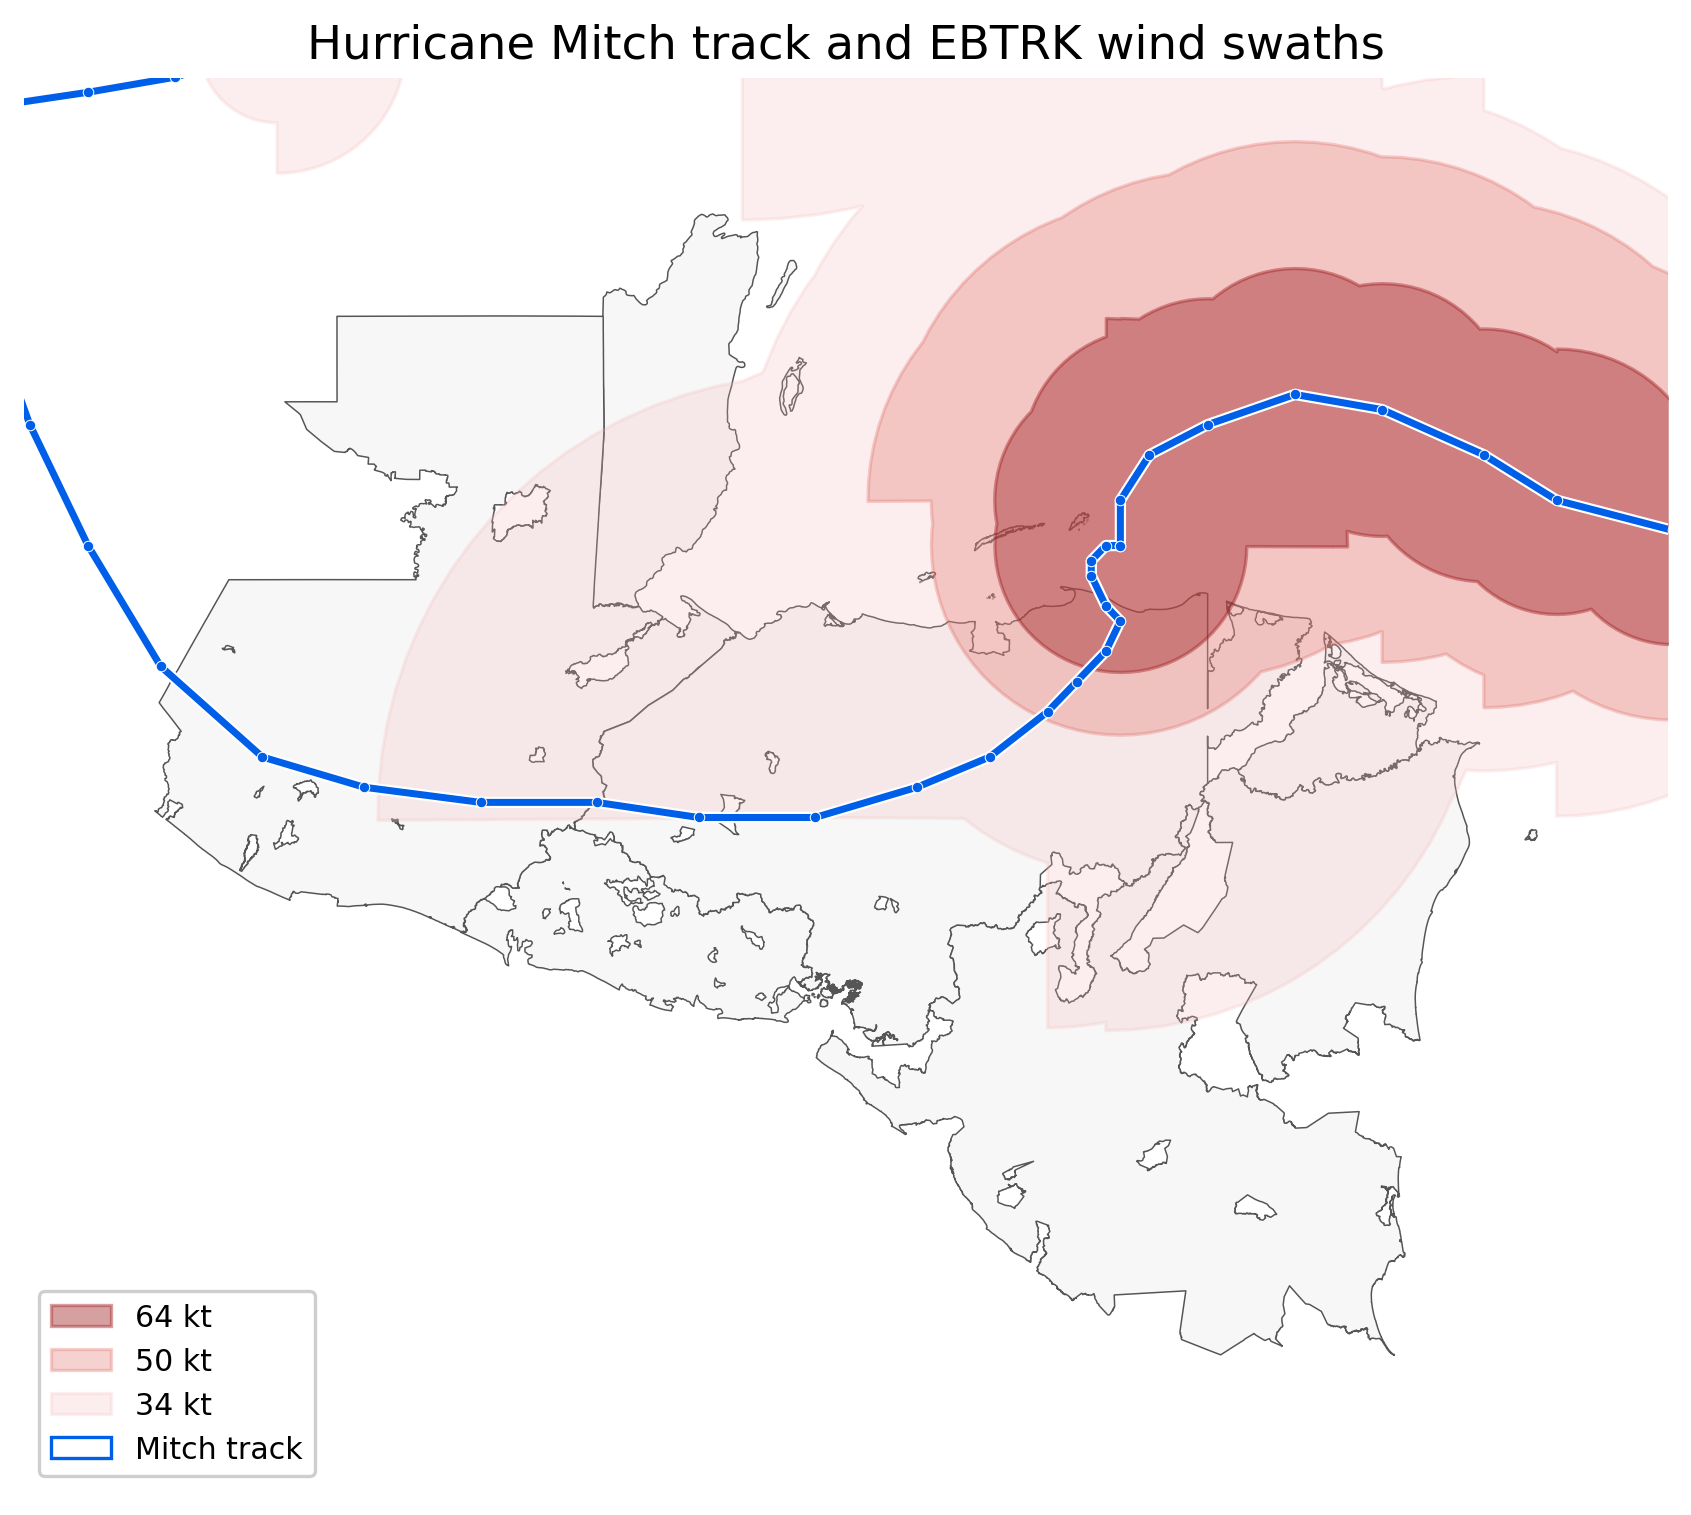
\includegraphics[width=0.72\linewidth]{Paper_Figures/data/exposure_maps/map_mitch_track_swaths.png}
\figurenotes{The figure shows Mitch's observed track over the selected Central American geography, with storm-total EBTRK wind swaths for 34-, 50-, and 64-knot winds. It is placed before the literature review to orient the reader to the spatial footprint before the empirical measures are introduced. Sources: NOAA IBTrACS, Extended Best Track wind radii, and GAUL/GeoBoundaries administrative boundaries.}
\end{figure}

% P4: Introduction, design, principal result, and roadmap
This paper estimates part of that loss. It assembles a municipality-year panel for Belize, El Salvador, Guatemala, Honduras, and Nicaragua that links DMSP-OLS nighttime lights from 1992 to 2013 to physically reconstructed measures of Hurricane Mitch exposure. A dynamic difference-in-differences design with municipality and year fixed effects compares nighttime-light paths in more- and less-exposed places. Two-year bins reduce annual DMSP noise, while annual specifications are reported in the appendix. The preferred wind estimates imply luminosity losses of roughly 10--20 percent during the first four post-Mitch years in municipalities with meaningful pre-Mitch light activity; unrestricted estimates are larger but noisier ranging from 50 to 60\%, and rainfall and mortality results are less robust. In a final section, the nightlight lost is liberally translated to an income loss through elasticities, the dwelling structure of wind treated municipalities is examined, and census data used to confirm the loss was temporary and concealed in the in-between of the three last available censuses: 2013, 2001, 1988 reaffirming the use of nightlight data, and its significant results. 

% PRESERVED REDUNDANCY: legacy summary paragraph retained for review but excluded from compilation.
% They will bear the brunt of their predicted increased frequency from anthropogenic climate change. How much can be lost informs how much should be spent, more so for countries with tight fiscal budgets, but identifying their causal effects remains a challenge. This paper estimates a portion of the causal loss. Creating a municipality-year panel, it examines the loss and recovery of Hurricane Mitch exposure (1998) in municipality-level night lights. A dynamic difference-in-differences framework allows the key questions of timing and recovery to be examined.

\subsection{Literature}
% P5: Literature, competing recovery paths
This paper contributes to three related literatures, first, to work on the economic impact and recovery of environmental disasters. A central question in that literature is whether disasters only temporarily interrupt growth, or whether shocks push economies durably below trend. Figure \ref{fig:recovery-hypotheses}, from Hsiang \& Jina, summarizes those competing expectations \citeyear{hsiang2014causal}. Proposed mechanisms range from creative destruction \parencite{skidmore2002promote} and ``build back better'' capital replacement \parencite{cuaresma2008natural,hallegatte2009can}, to recovery through transfers and migration \parencite{yang2008coping}, and finally to persistent losses with no full rebound \parencite{field2012managing}. For their own estimate, Hsiang and Jina reconstruct cyclone exposure for 6,700 storms and find that incomes fall relative to pre-disaster trends and do not recover within twenty years, with losses magnified in places less historically exposed to cyclones \parencite{hsiang2014causal,hsiang2012adaptation}. 

\begin{figure}[htbp]
\centering
\caption{\label{fig:recovery-hypotheses}Disaster recovery hypotheses in the literature}
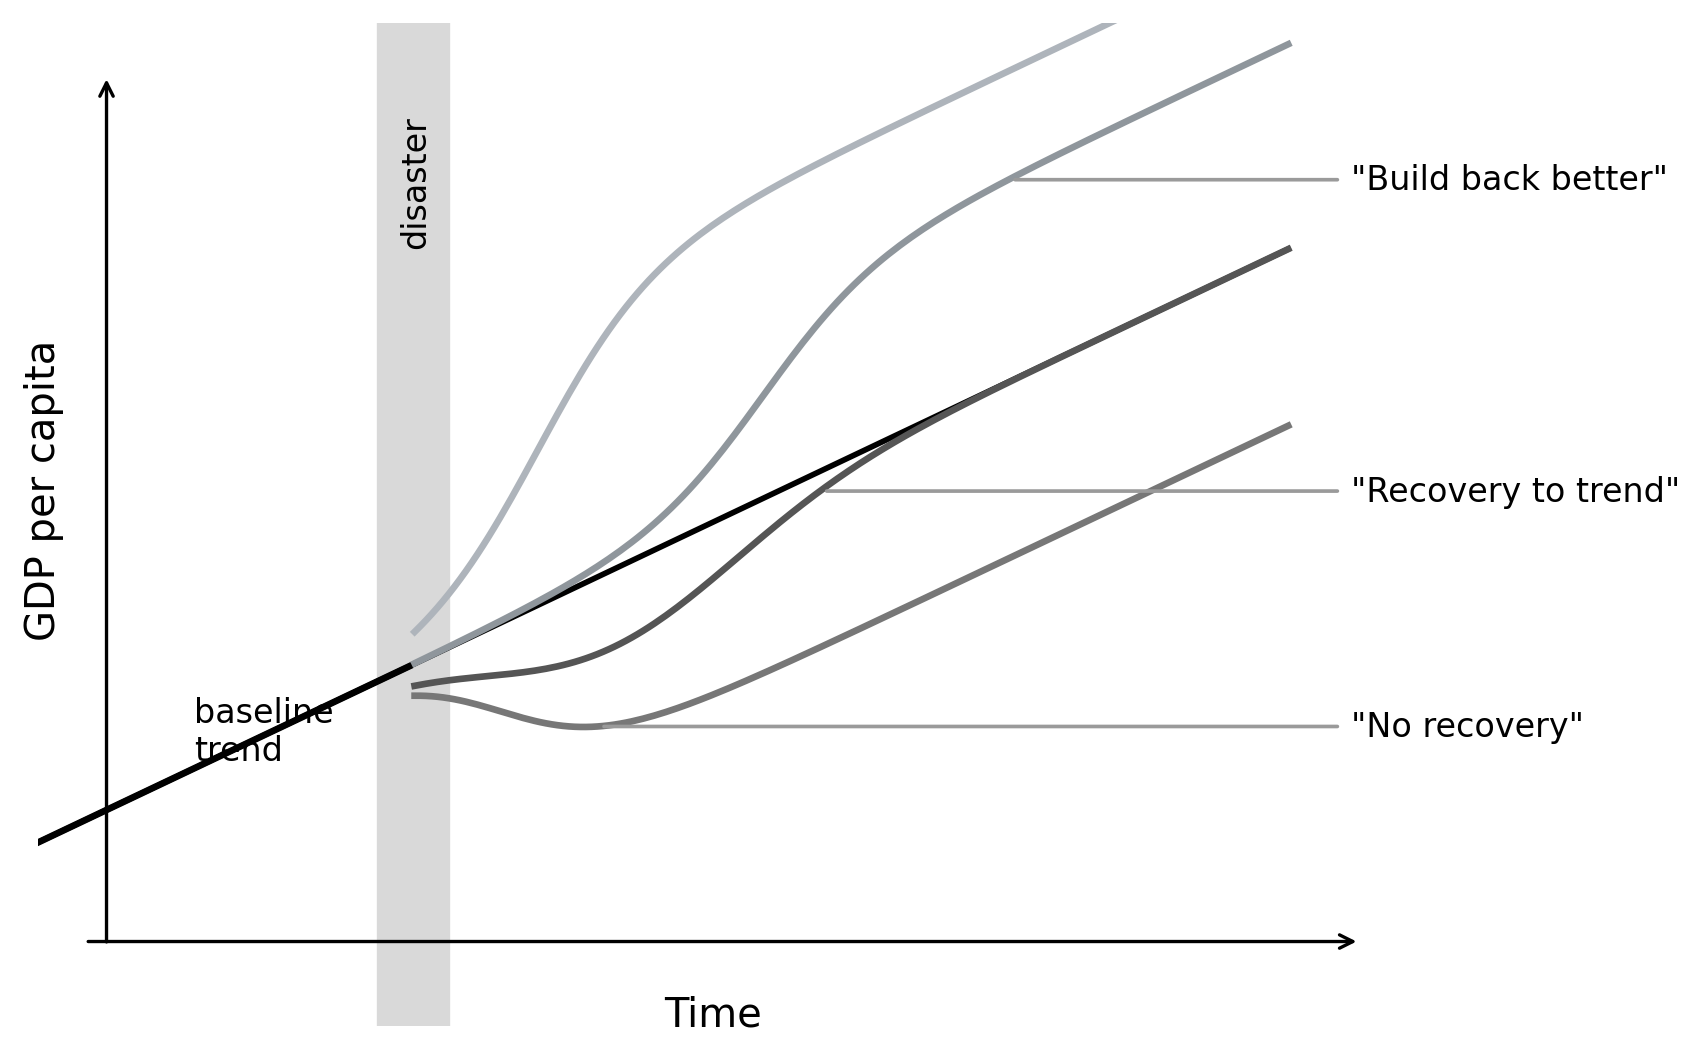
\includegraphics[width=0.72\linewidth]{Paper_Figures/data/literature/recovery_hypotheses.png}
\figurenotes{The schematic summarizes the range of post-disaster paths discussed in the disaster-growth literature: creative destruction, building back better, recovery to trend, and no recovery.}
\end{figure}

% P6: Literature, closest regional nighttime-lights study
Ishizawa, Miranda, and Zhang (2017) provide the closest geographic and topical parallel to this study, as Hurricane Mitch serves as the sole event in their major hurricane category in their study of Central American windstorms \citeyear{ishizawa2017windstorms}. Using monthly nighttime lights at a 1 km² resolution, they identify a 17\% average luminosity decrease over the first twelve months, followed by an eighteen-month recovery that roughly offsets the initial drop \parencite{ishizawa2017windstorms}. In contrast, I aggregate the yearly series of the same nightlight data to the municipality level. Their monthly granularity is constrained by an average of only five daily cloud-free observations per month—a factor they find significantly correlated with their results, whereas the yearly data have cloud-free observations ranging from 39 to 55 for satellites during Mitch years. Nevertheless, my analysis finds a similar temporary disruption, identifying a persistent four-year (48-month) impact rather than their 30-month window, reinforcing the validity of both studies. 

% P7: Literature, Mitch household evidence and contribution
Second and related, this paper contributes to the literature on Hurricane Mitch specifically which has principally shown the storm's effect through localized rural surveys in Honduras. Specifically, the three studies below use the 1999 IFPRI/PRAF nutritional survey of 2,398 households and a separate 1994–2001 land-reform panel of 850 households.  Morris et al.\ document severe post-Mitch losses among the rural poor within six to nine months of the storm, including a 5.5 percentage point rise in rural poverty, and losses of productive assets \parencite{morris2002mitch}. Gitter and Barham show that, using a sample of 387 children from the land-reform panel, Mitch reduced age-adjusted schooling (SAGE) scores by approximately 25 points in the three years following the disaster among credit-constrained households \parencite{gitter2007credit}. Carter et al.\, using that same panel effort, identify an asset threshold of \$250, finding that severe environmental shocks can push households below critical asset thresholds and onto divergent, lower-level recovery paths that persisted at least thirty months after the event. I move beyond the constraints of these localized survey efforts—which were restricted to rural sub-samples, to analyze Mitch’s economic footprint at a spatial and temporal resolution previously impossible. 

% DRAFT NOTE (preserved): The old text incorrectly described Ishizawa's units as 1 x 1 grids and the 18 months as a period without recovery.

% P8: Literature, measurement scale and physical exposure
Finally, the paper contributes to discussions around how disasters should be measured and what scale they should be studied. If the unit of analysis is too broad, it risks missing the local mechanisms through which storms do damage; if it is too narrow, it risks mistaking local noise for the disaster itself. Hsiang and Jina's previously discussed country-level windstorm design necessarily trades away sub-national heterogeneity in mechanism, especially for storms like Mitch whose destructiveness depended not only on wind, but flooding and local infrastructure vulnerability. More spatially disaggregated work can push in the other direction. Gandhi et al.\ combine geocoded flood events, TerraClimate precipitation, and monthly VIIRS night lights for 9,468 cities to study short-run losses and recovery, showing that floods depress night lights more strongly and for longer in poorer places \parencite{gandhi2022adapting}. To build a hypothetical from their example, city-level floods may be part of a regional weather pattern experienced by the entire country; if flooded cities are compared against unflooded rural areas within the same nation, the resulting estimates will be biased. This is a possible threat to my study if Mitch depressed income or electrification across all my control municipalities listed below. Mean stable lights in Figure \ref{fig:ntl-1998-one-page} suggest this is not the case, nor do they show a lag at the Honduran national level, motivating my approach at the sub-national scale still larger than household surveys.
% DRAFT NOTE (preserved): This sentence replaces the bracketed revision instruction in the old draft.

\section{Data}

% P9: Data, sample and geography
To isolate the economic impact and recovery of Mitch, I combine DMSP-OLS night lights from 1992 through 2013 with 1998 Mitch exposure measures across Central America for a municipality-year panel. Municipalities are all available GAUL-coded municipalities in Belize, El Salvador, Guatemala, Honduras, and Nicaragua. Costa Rica and Panama are omitted as their development trajectories made them less defensible controls for the others, which form a loose block \footnote{The latter being inseparable from logistics and the Canal, and Costa Rica from high-skill export and services, culminating in its being denominated the only ``high-income'' country in the region in 2025 \parencite{worldbank2025countrygroups}. All the rest share development models more dependent on agriculture, low-value manufacturing, remittances, and informality. Belize is somewhat of an outlier in the sample as the only British-colonized state, but it is retained as its agricultural and remittance linkages are aligned.}. There are 1,053 GAUL-coded selected-country NTL municipalities in the source crosswalk, with 996 ending up in the final corrected municipality-year panel. The units that do not enter are cases where no conservative one-to-one polygon exists in the current GeoBoundaries file, such as lake units, island fragments, administrative placeholders, or named units without a unique ADM2 polygon. Table 1 reports summary statistics for the outcome described below and the treated and control municipality shares for each exposure measure.

\begin{table}[htbp]
\centering
\caption{\label{tab:exposure-summary}Data and exposure summary statistics}
\begingroup
\scriptsize
\setlength{\tabcolsep}{3pt}
\resizebox{\linewidth}{!}{%
\begin{tabular}{lrrrrrrr}
\toprule
\multicolumn{8}{l}{\emph{Dependent Variable: Nightlights}} \\
Name & Mean & SD & P10 & P25 & P50 & P75 & P90 \\
\midrule
DMSP-OLS stable lights & 587.4 & 1,368 & 0.361373 & 66.61 & 218.0 & 588.0 & 1,359 \\
DMSP-OLS stable lights pre-Mitch & 357.2 & 1,057 & 0.060131 & 13.62 & 101.79 & 334.9 & 774.8 \\
\addlinespace[0.45em]
\multicolumn{8}{l}{\emph{Independent Variable: Mitch Exposure Measures}} \\
Name & Source & Amount treated & \begin{tabular}{@{}c@{}}Treated at or above\\pre-Mitch median\end{tabular} & Amount control & \begin{tabular}{@{}c@{}}Controls at or above\\pre-Mitch median\end{tabular} &  &  \\
\midrule
64 kt winds & Extended Best Track & 9 & 4 & 987 & 494 & & \\
50 kt winds & Extended Best Track & 16 & 8 & 980 & 490 & & \\
34 kt winds & Extended Best Track & 258 & 109 & 738 & 389 & & \\
Top 10\% maximum rainfall anomaly & CHIRPS & 94 & 58 & 902 & 440 & & \\
Top 10\% deaths per capita (state*) & Government Reports & 8* & 8* & 64* & 63* & & \\
\bottomrule
\end{tabular}

}
\endgroup
\tablenotes{The table reports reader-facing municipality counts for the retained selected-country geography. EBTRK treatment counts use the preferred rule that at least 50 percent of municipal area is inside the storm-total swath. The CHIRPS specification is the standalone top decile of municipality-level maximum rainfall anomaly; deaths per capita is measured at the state or department level. Sources: NOAA DMSP-OLS stable lights, GAUL administrative units, Extended Best Track wind radii, CHIRPS rainfall, and state-level Mitch impact data.}
\end{table}

\subsection{Outcome: DMSP-OLS nightlights}
% P10: Data, why satellite and census data are used
The use of satellite data for night lights sidesteps issues of data availability in a developing context. Honduras's last census was in 2013 and is briefly used as a robustness check in the results \footnote{The available census years are 1961, 1974, 1988, 2001, and 2013}, while its annual household survey (EPHPM) is representative at the 5\% level only for the two biggest cities and an overgeneralized 'countryside'. \parencite{ipumsinternational2025}.
From these limitations, recent economics work has used night light data as a proxy for economic activity \parencite{donaldson2016view, henderson2011bright}. The approach is rooted in the assumption that light is a normal good, as income and production increase, the demand for and emission of visible light follows a stable relationship.  Ishizawa et al. (2017), for example, provide regional structural elasticities of real GDP with respect to nighttime lights for Central America between 0.158 and 0.233 by regressing real GDP on the DMSP-OLS series described below. It is important to remember the elasticities are suggestive and night lights remain a measure of electrification and infrastructure, not income itself. Nevertheless, because satellites provide uniform spatial sampling regardless of national borders at extremely granular levels, they enable the study of economic activity in geographic units for which traditional data are frequently nonexistent, and where disaster damage reports may be inconsistently measured \parencite{donaldson2016view, henderson2011bright}.

% P11: Data, nightlight construction and outcome
Nightlight data come from the Defense Meteorological Satellite Program (DMSP) Operational Linescan System (OLS) covering 1992 to 2013. DMSP data were extracted from Google Earth Engine by assigning roughly 1 x 1 km pixels to GAUL-coded municipalities as shown in Figure \ref{fig:ntl-1998-one-page}. The main outcome is \textit{stable\_sum}, the sum of pixel values, ranging from 0 to a saturation point of 63, in a municipality-year. Table \ref{tab:exposure-summary} reports \textit{stable\_sum} over the coverage years and in the pre-Mitch period. In the empirical specifications, \textit{stable\_sum} is transformed as \textit{log(1 + stable\_sum)} to retain zero-light observations, 96 of 996 municipalities in the pre-Mitch period, while reducing the influence of very bright municipalities. 

% P12: Data, DMSP limitations and annual timing
As has also been noted, the older DMSP series of nightlight data has its limitations. Relative to alternatives such as VIIRS, which begins in 2012, DMSP is coarse, suffers from top-coding in bright places, exhibits blooming and blur, lacks on-board calibration as shown in Figure \ref{fig:ntl-1998-one-page} over the six satellites used in the sample, and can be especially noisy for small or low-density areas \parencite{gibson2021which}. Further, as a yearly product, DMSP's coarseness means the 1998 DMSP municipality year observations are a mix of pre- and post-Mitch composites with 1999 being the first clean year. Early implementations of monthly DMSP specifications proved noisy, with whole regional swaths being cloud covered for certain months. The Visible Infrared Imaging Radiometer Suite (VIIRS) on the Suomi National Polar-orbiting Partnership satellite gets around many of these issues by offering a monthly product; however, it does not cover Mitch years \parencite{gibson2020night,gibson2021which,elvidge2017viirs}.

% P13: Data, pre-Mitch luminosity sample
The preferred sample retains municipalities whose pre-Mitch mean \texttt{stable\_sum} is at or above the pre-Mitch sample median (101.79). This filter limits the mechanical sensitivity of $\log(1+NTL)$ near zero and addresses the instability of DMSP-OLS measurement in dim, rural settings, where low-intensity lighting often falls below the sensor's detection threshold and can produce a weak or even negative relationship between lights and rural economic activity \parencite{gibson2021which}. For example, an increase from 5 to 15 stable-light units changes $\log(1+NTL)$ by $\log(16)-\log(6)=0.98$, which would resemble a large economic boom despite an absolute increase of only ten units. Consistent with that concern, the unfiltered wind specifications imply substantially larger losses. Empirically, 496 of the 498 municipalities retained by the median cutoff have a pre-Mitch mean-to-standard-deviation ratio of at least one, while 99 percent of municipalities failing that stability criterion lie below the cutoff.\footnote{That is, where $\mathrm{SNR}_i \geq 1$, where $\mathrm{SNR}_i \equiv \overline{NTL}_{i,\mathrm{pre}}/\sigma(NTL_{i,\mathrm{pre}})$.}



\begin{figure}[p]
\centering
\caption{\label{fig:ntl-1998-one-page}DMSP-OLS nighttime lights in the Mitch year}
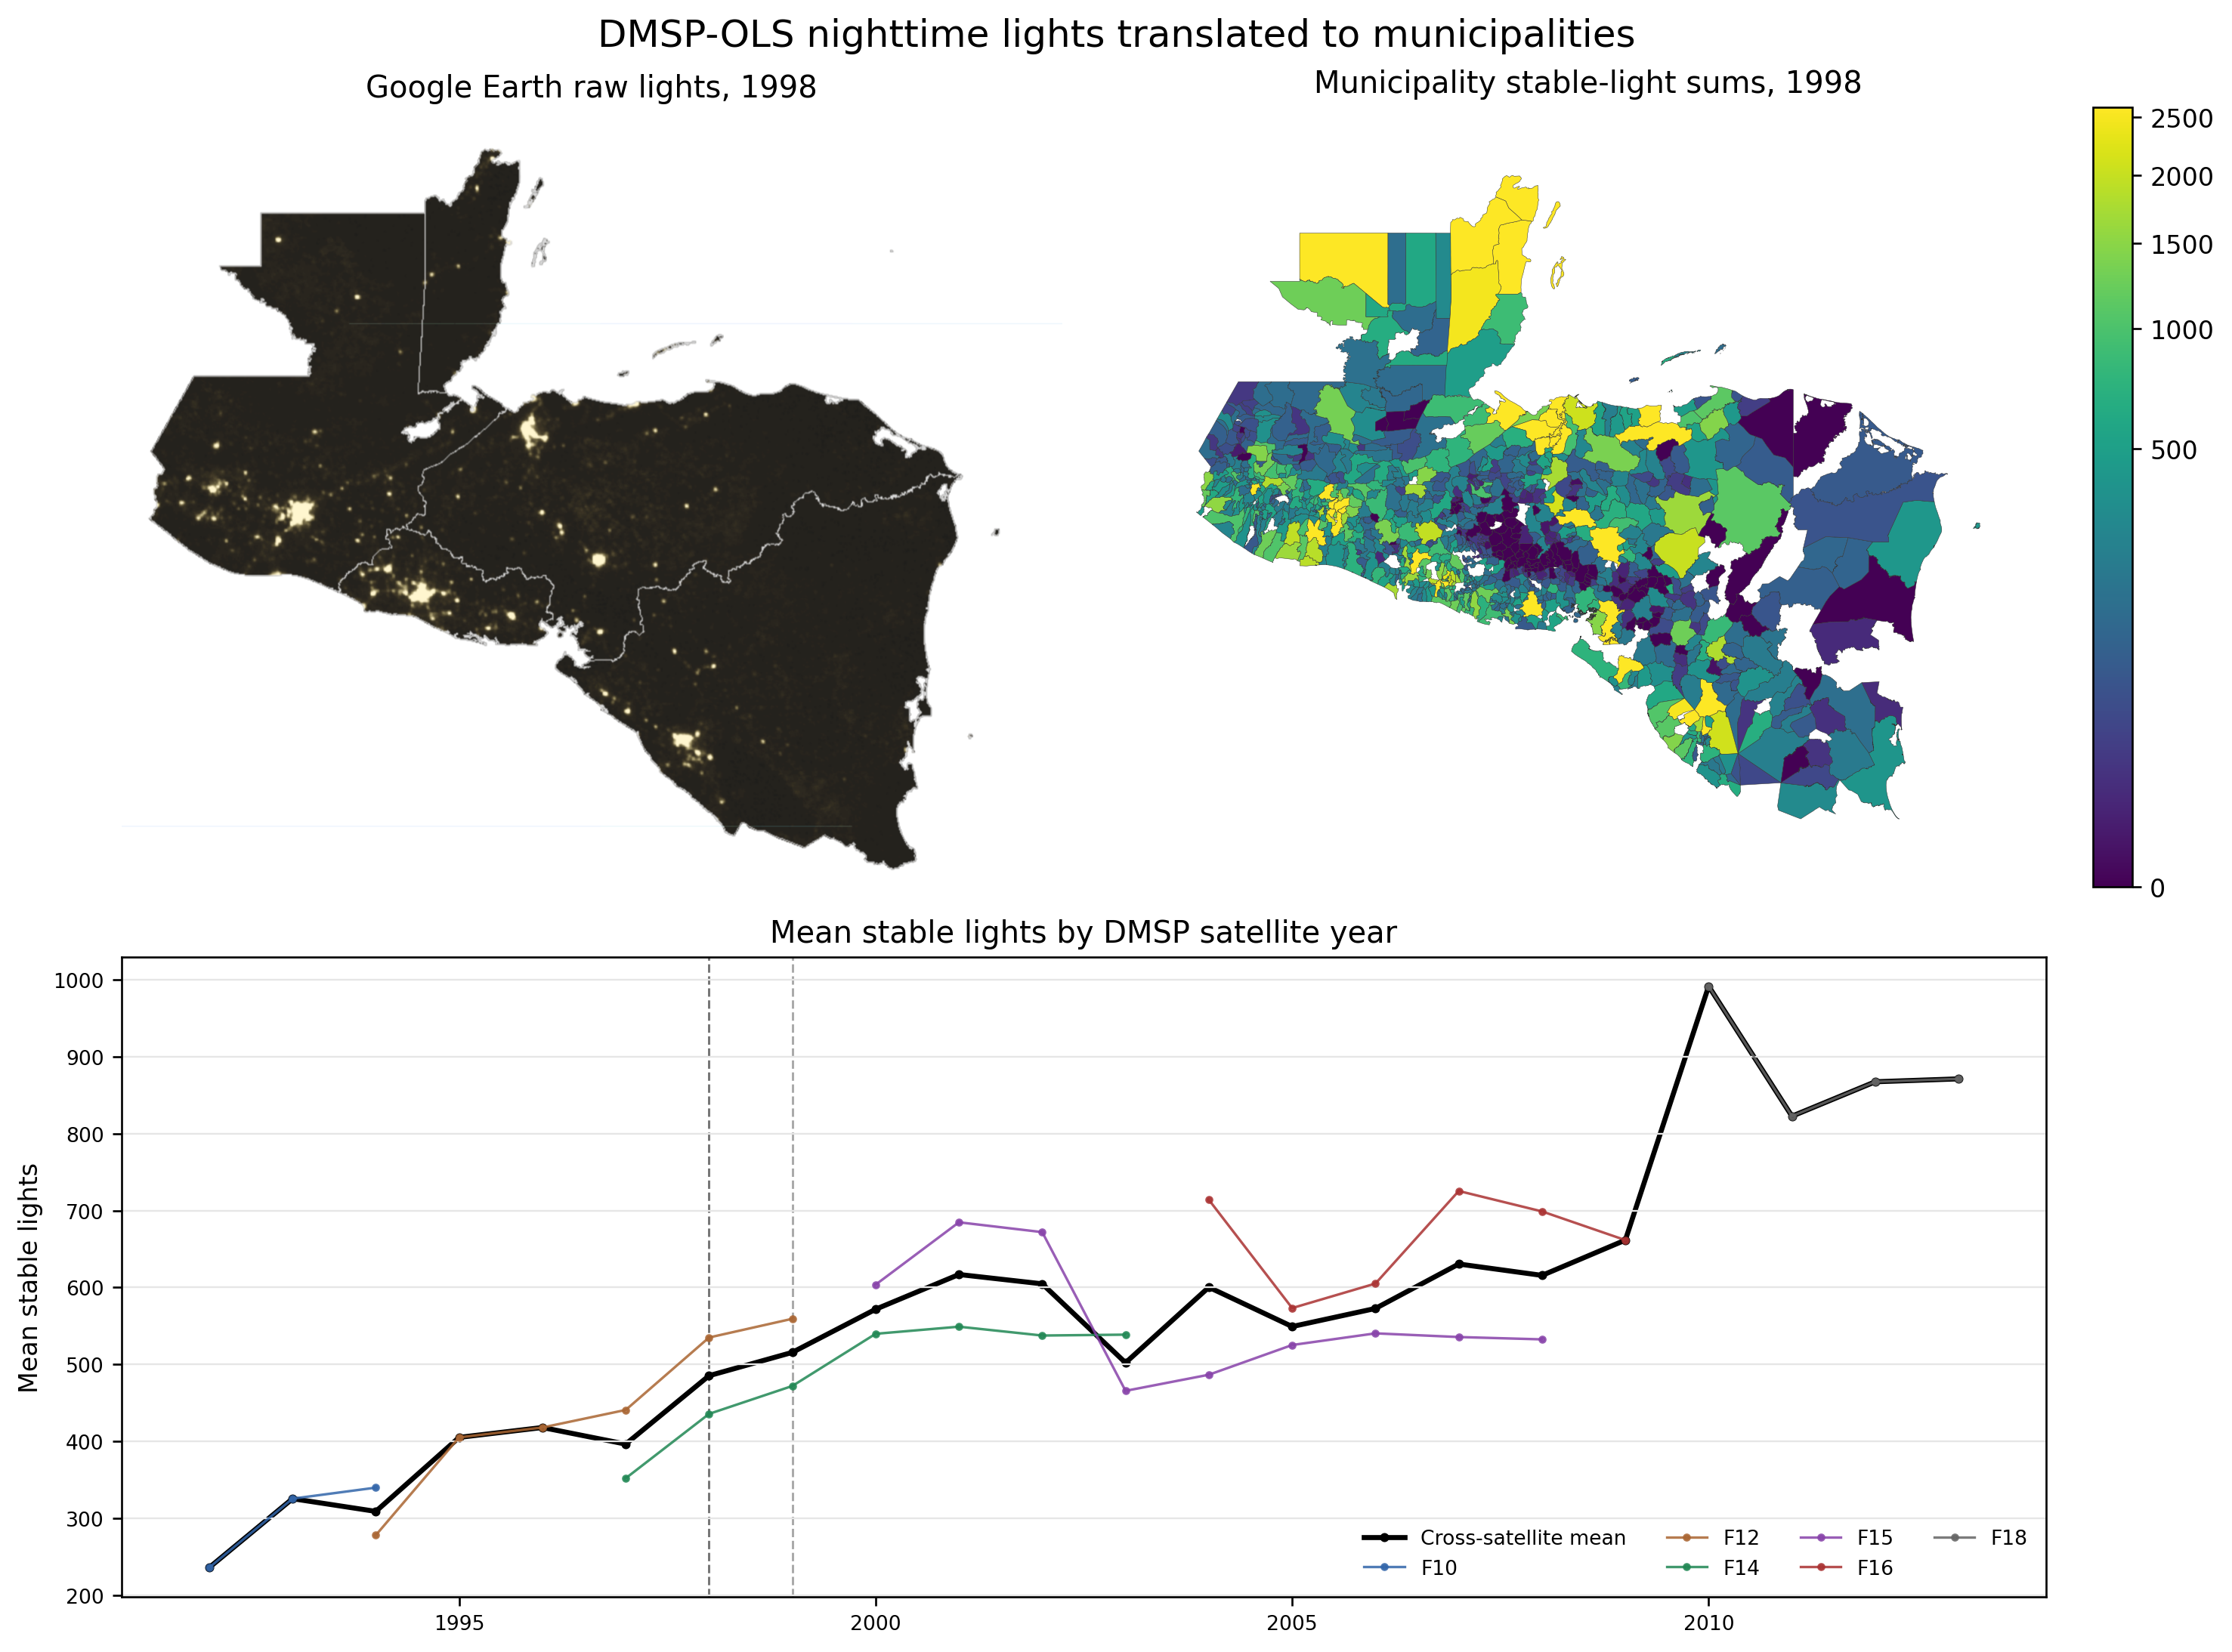
\includegraphics[width=0.96\linewidth]{Paper_Figures/data/ntl_maps/ntl_1998_one_page.png}
\widefigurenotes{The left panel shows the Google Earth raw-light image for the retained Central American geography. The right panel translates the same 1998 DMSP-OLS lights into municipality stable-light sums using the regression geography. The bottom panel reports mean stable lights by DMSP satellite-year, with the cross-satellite mean drawn behind the individual satellite series so overlapping single-satellite years remain visible. Source: NOAA DMSP-OLS stable lights, extracted over GAUL/GeoBoundaries administrative units.}
\end{figure}

\subsection{Mitch Exposure Measures}

% P14: Data, Mitch exposure families
I measure Hurricane Mitch exposure as reconstructed wind exposure, extreme rainfall exposure, and reported mortality severity. Wind measures provide the most physically grounded and spatially explicit exposure family in the paper, though they cannot capture the full hydrological and social geography of Mitch's damage. The four treatment definitions, which municipalities they treat, and which of these are excluded from the pre-Mitch sample median filter are visualized in Figure \ref{fig:ebtrk-threshold-map}. Treated and control counts are reported in Table \ref{tab:exposure-summary}.

\begin{figure}[p]
\centering
\caption{\label{fig:ebtrk-threshold-map}Primary Mitch treatment maps}
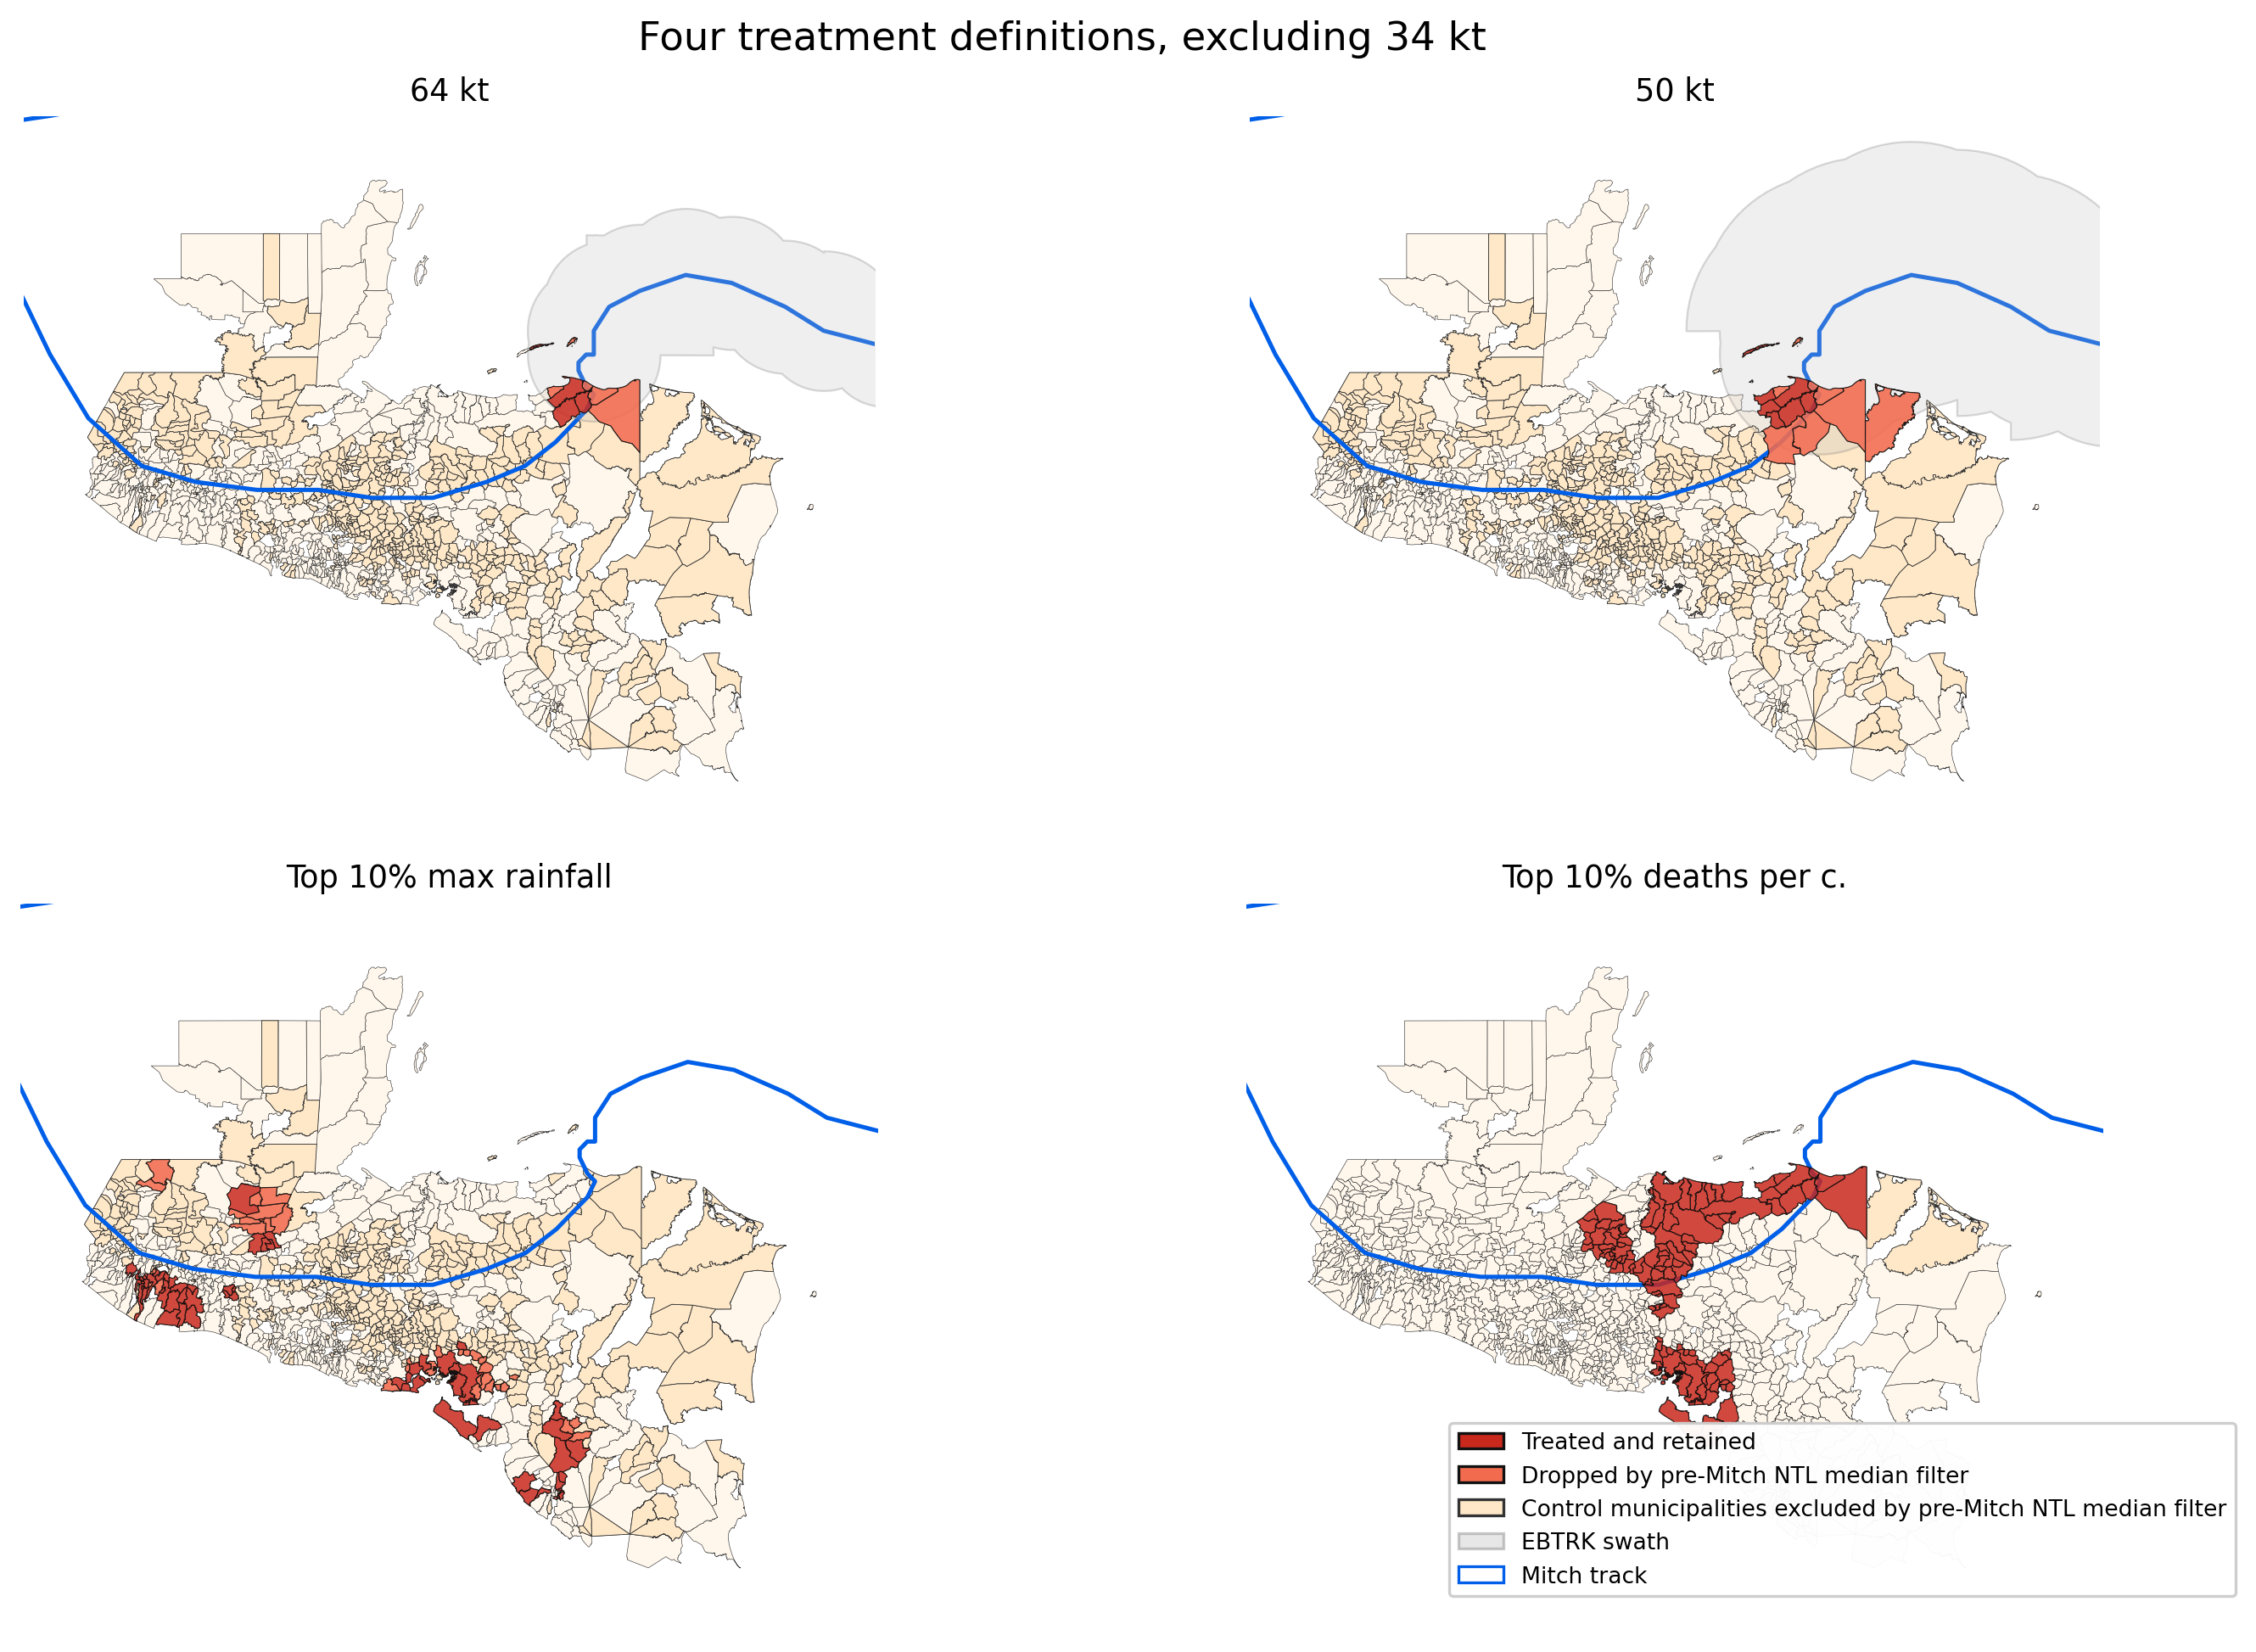
\includegraphics[width=\linewidth]{Paper_Figures/data/exposure_maps/map_four_treatments_no34.png}
\figurenotes{The panels show the four main binary treatment definitions emphasized in the paper, excluding the broad 34-knot specification. Red municipalities are treated and retained under the pre-Mitch median luminosity filter; orange municipalities are treated but dropped under that filter. Wind panels also show the exact EBTRK swath overlay and Mitch track. The binary EBTRK rule is that at least 50 percent of municipal area is covered by the relevant storm-total swath. Sources: NOAA IBTrACS, Extended Best Track wind radii, GAUL administrative boundaries, and the project assignment crosswalk.}
\end{figure}

\subsubsection{Best and Extended Best Track Reconstruction}

% P15: Data, Best Track source and reconstruction

Mitch's track and windstorm are constructed from Best Track and Extended Best Track data from the National Oceanic and Atmospheric Administration (NOAA) accessed through the harmonized Archive for Climate Stewardship (IBTrACS). Best-track records are post-storm meteorological assessments of a cyclone's position, central pressure, and, where available, size \parencite{landsea2013atlantic}. They utilize all best available evidence including satellite but also aircraft reconnaissance, scatterometer, radar and more reviewed by specialists to produce a ``best track''. Best Track itself does not include Atlantic wind radii before 2004 so I supplement its storm-center positions and intensities with Extended Best Track wind-radius information. Extended Best Track gives wind radii for the 34-, 50-, and 64-knot thresholds, which I use to construct wind swaths and intersect those with municipality polygons. On the Beaufort scale, 34 knots mark gale-force winds, 50 knots mark storm-force winds at which damage begins to be expected, and 64+ knots mark hurricane-force winds. Wind damage rises nonlinearly between them. \footnote{In particular, the dynamic pressure applied to structures increases approximately with the square of velocity, so moving from 34 to 50 knots more than doubles the wind loading relevant for infrastructure \parencite{nhc2017product}}. From this, I report 50- and 64-knot thresholds as main treatments and place 34-knot exposure and event studies in the appendix. For each threshold I use a binary municipality-level exposure measure equal to one if at least half of the municipal area is covered by the swath. Extended Best Track also permits an area-share measure, but this paper does not use a continuous exposure specification.

\subsubsection{CHIRPS, Deaths per Capita, and Census Data}

% P16: Data, rainfall exposure
Much of Mitch's destructiveness came not only from wind, but also extreme rainfall and flooding. After making landfall, the storm effectively stalled over Honduras before meandering into the wider region. The paper also uses CHIRPS precipitation as a separate physical exposure measure. CHIRPS provides gridded rainfall estimates that can be aggregated to the same municipality geography as the DMSP-OLS outcome. I use the municipality-level maximum rainfall during the Mitch window minus historical averages and define the main CHIRPS treatment as the top decile of that anomaly within the retained regional sample. This measure is best interpreted as a rainfall-intensity proxy, not a direct flood-depth measure. It captures unusually high precipitation over the municipality, but local flooding also depends on infrastructure, soil retention, or the wider geography. 

\begin{figure}[htbp]
\centering
\caption{\label{fig:chirps-excess-water-volume}Hurricane Mitch precipitation volume above the calendar-day climatology}
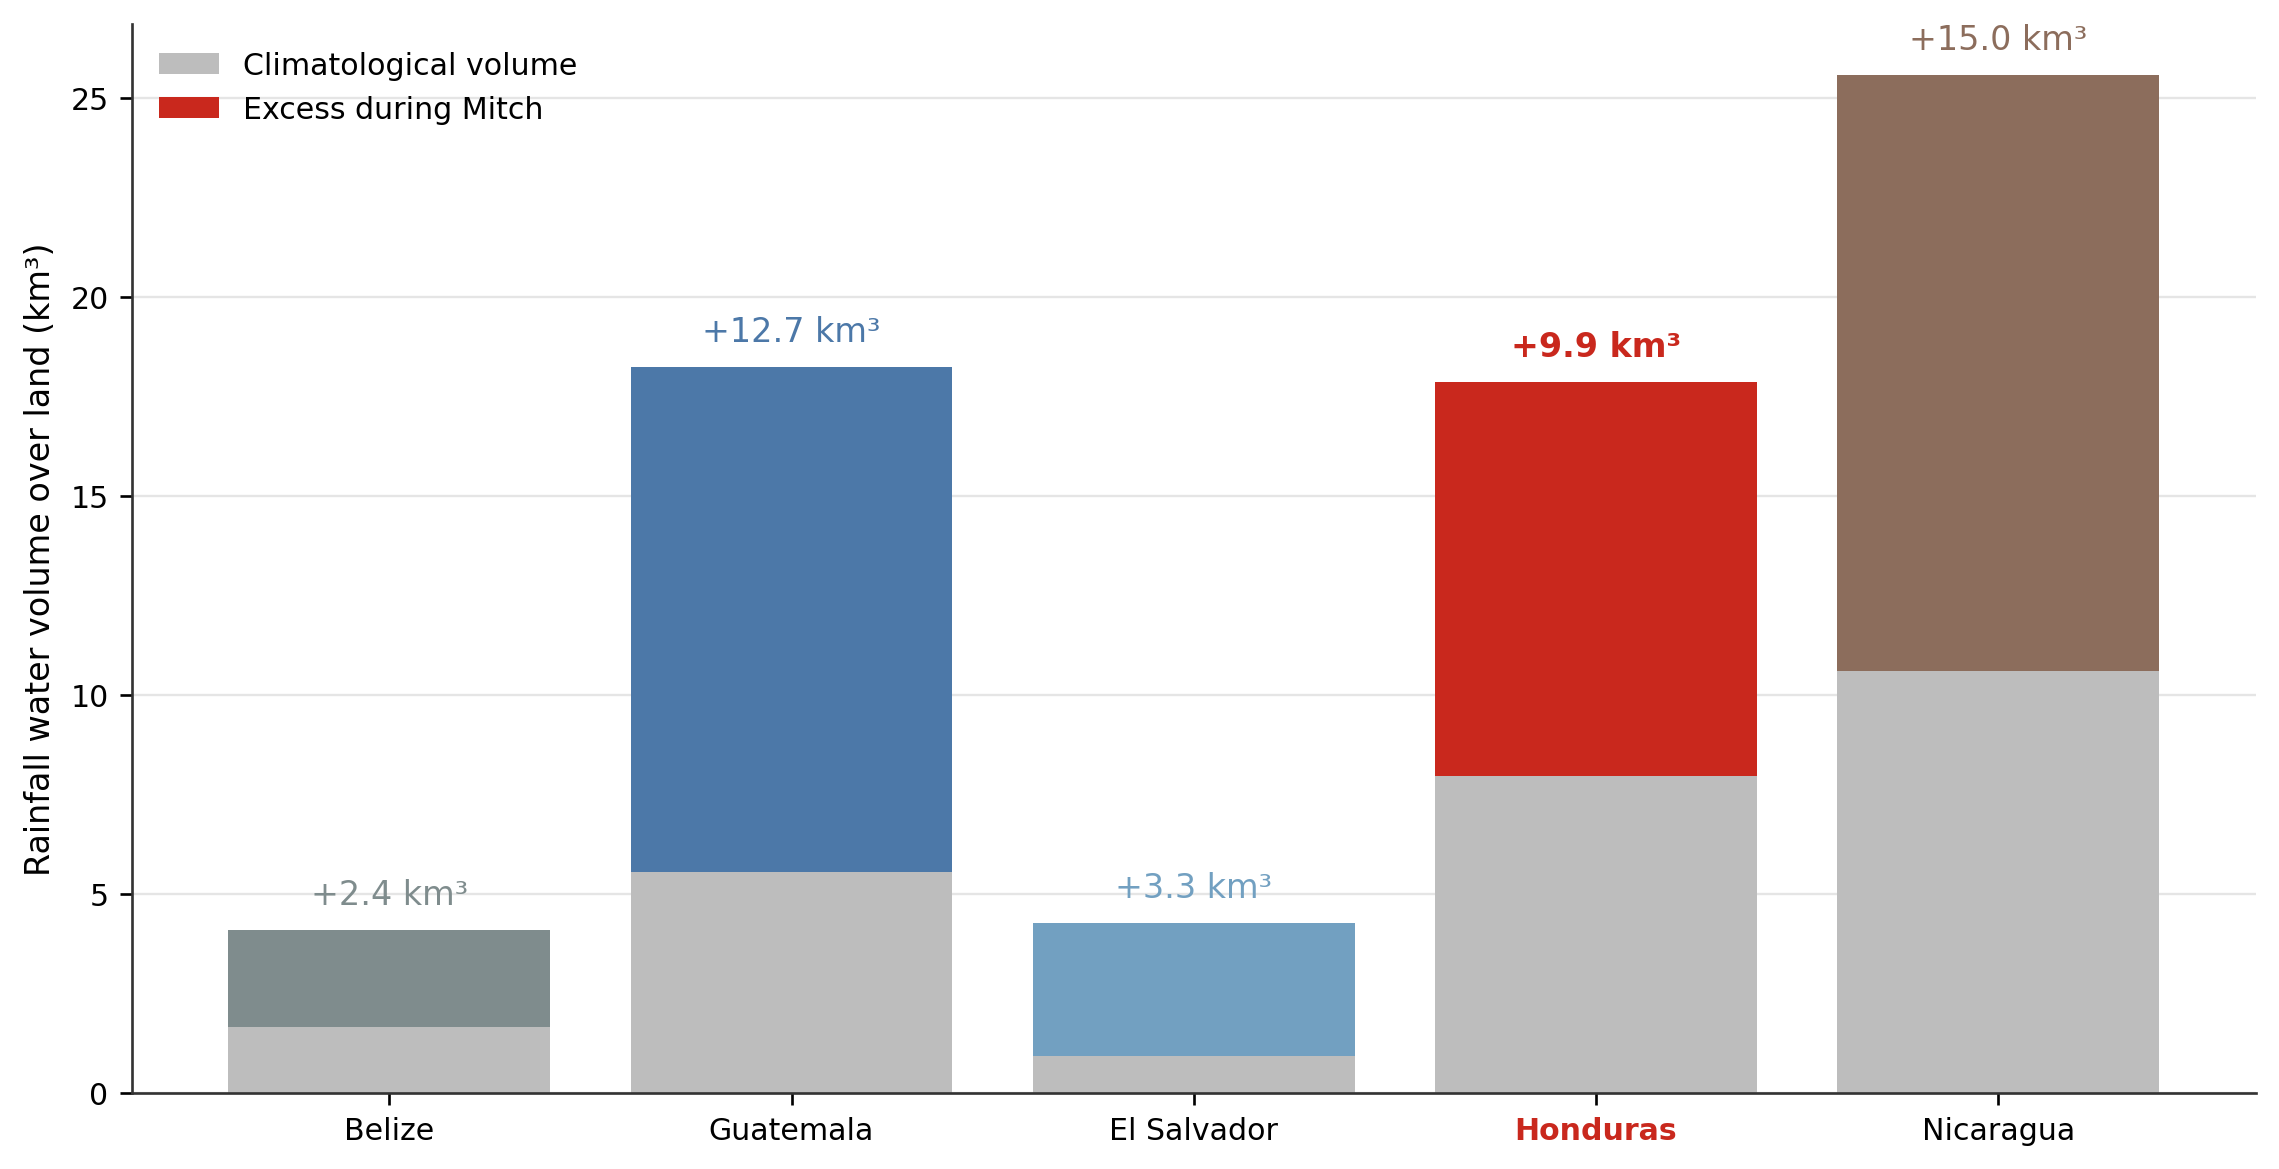
\includegraphics[width=0.82\linewidth]{Paper_Figures/data/CHIRPS/06_excess_precipitation_water_volume.png}
\figurenotes{The figure compares CHIRPS precipitation volume over land during October 27--November 4, 1998 with the supplied 1981-present mean for the same calendar days. Rainfall depth is converted to cubic kilometers using geodesic raster-cell areas and fractional country coverage; one millimeter over one square kilometer equals $10^{-6}$ cubic kilometers. ``Excess'' is the observed Mitch-period volume minus that climatological volume. It is precipitation volume, not measured runoff, floodwater, or a return-period estimate. Source: CHIRPS daily precipitation and author's calculations.}
\end{figure}

% P17: Data, mortality as downstream severity
As an alternative that incorporates geographic vulnerability, I include a deaths-per-capita treatment. The mortality data are reported at the first administrative level, so this is the only specification that changes the unit of analysis from municipality to the department level. I compute deaths per capita at that level, assign the corresponding top-decile indicator to all municipalities inside the department for mapping, and aggregate nighttime lights to a department-year panel for the regression. Unlike the wind and rainfall specifications, the deaths-per-capita treatment works backward from realized damage and combines physical exposure with vulnerability and settlement patterns. Its overlap with CHIRPS around the Gulf of Fonseca between Honduras and Nicaragua, together with the fact that Mitch first produced Temporary Protected Status for Nicaraguans, who were not hit by 50 kt+ winds is strong evidence of the damage the strict wind exposure misses. 

% P18: Data, Honduran census robustness sample
Finally, I use IPUMS International harmonized Honduran census microdata to describe the 50-knot groups and provide low-frequency robustness checks. Because GEO2\_HN groups sometimes combine legal municipalities, treatment is assigned at the harmonized-group level. The preferred census DiDs retain the three groups containing 12 treated and no untreated municipalities and exclude mixed groups. Comparable household asset measures are available in 1988, 2001, and 2013 \parencite{ipumsinternational2025}.

\section{Empirical Strategy}

% P19: Empirical strategy, equation and units
Having constructed treatment and comparison units from Hurricane Mitch exposure, I estimate dynamic difference-in-differences regressions of the form
\begin{equation}
    \log(1+NTL_{it})
    =
    \sum_{\substack{\tau=92'\text{--}93'\\ \tau\neq 96'\text{--}97'}}^{12'\text{--}13'}
    \beta_{\tau}
    \left(Exposure_i^{1998}\times \mathbf{1}[t\in \tau]\right)
    +\alpha_i+\lambda_t+\varepsilon_{it}.
\end{equation}
Here $i$ indexes the estimation unit, municipality or department, and $t$ indexes calendar years. The dependent variable is $\log(1+NTL_{it})$, where $NTL_{it}$ is DMSP-OLS stable nighttime lights. Nightlights are logged to reduce the influence of very bright municipalities and make coefficients more easily interpretable as percent changes. The variable $Exposure_i^{1998}$ is the treatment measure induced by Hurricane Mitch exposure, and $\mathbf{1}[t\in\tau]$ equals one when year $t$ falls in two-year bin $\tau$. Two-year bins reduce annual DMSP noise, unbinned visual specifications are reported in the appendix, and the omitted reference period is 1996--1997 before Mitch. 

% P20: Empirical strategy, coefficient and fixed-effects interpretation
The key coefficients in equation (1) are the time-varying $\beta_\tau$'s, which capture how much lower or higher treated units were after removing permanent place differences, common year shocks, relative to the treated-control difference immediately before Mitch. If the comparison group is credible, the pre-Mitch $\beta_\tau$s should be close to zero, while the post-Mitch $\beta_\tau$s reflect post-Mitch differences between units exposed to Mitch in 1998 and the comparison units.\footnote{More precisely, $\beta_\tau$ captures the residual difference-in-differences in $\log(1+\text{nighttime lights})$ between exposed and unexposed units in two-year bin $\tau$, relative to their 1996--1997 exposed-control gap, after partialling out unit fixed effects and calendar-year fixed effects. Because the dependent variable is in log levels rather than growth rates, $\beta_\tau$ is measured in log points; $100\times(\exp(\beta_\tau)-1)$ gives the corresponding approximate percentage difference.} Unit fixed effects, $\alpha_i$, absorb time-invariant differences across estimation units, while year fixed effects, $\lambda_t$, absorb annual shocks common to the retained sample, which is crucial for DMSP-OLS because it accounts for the on-board calibration issues between satellites previously shown in Figure \ref{fig:ntl-1998-one-page}. Standard errors are clustered by the estimation unit.

\section{Results}

% P21: Results, four-year dip and display roadmap
Across treatment specifications, there is an approximately four-year dip in night lights relative to the pre-Mitch treated-control difference. The loss is causal as there are parcel trends given the pre-Mitch coefficients are not statistically distinguishable from zero though the 64-knot group has the weakest case. Figures \ref{fig:unit-fe-dynamic} and \ref{fig:event-ebtrk-thresholds} are shown to first display the clearest visual logic of the four-year dip and then the most defensible magnitude of its loss. 

As visualized in Figure \ref{fig:unit-fe-dynamic} wind and mortality-treated areas separate from their comparison groups after Mitch with the gap closing by the 2002--2003 bin. The rainfall exposure measures behave show no temporally consistent treated-control decline. Per Figure \ref{fig:event-ebtrk-thresholds} which reports magnitudes with year fixed effects to protect against common shocks, such as lack of satellite calibration, alongside the pre-Mitch nightlight filter to protect against near-zero sensitivity and instability, the luminosity losses are roughly $-10.3\%$ in 1998--1999 and $-20.5\%$ in 2000--2001. The 50-knot specification is similar, with implied losses of $-15.5\%$ and $-20.4\%$. Both wind estimates are statistically significant at the 1 percent level. As reported in Table \ref{tab:ebtrk-binary-reg}, the 64-knot pre-Mitch nightlight unfiltered estimates are large and imprecise, while the 50-knot estimates imply declines of approximately 61 and 68 percent, significant at 10 and 5 percent levels. The top-decile rainfall specification shows a significant loss in the first post-Mitch period, but the pattern disappears in 2000--2001 and turns positive with the luminosity filter. 

% P22: Results, unit-fixed-effects display
\begin{figure}[p]
\centering
\caption{\label{fig:unit-fe-dynamic}Two-year nighttime-light paths with unit fixed effects}
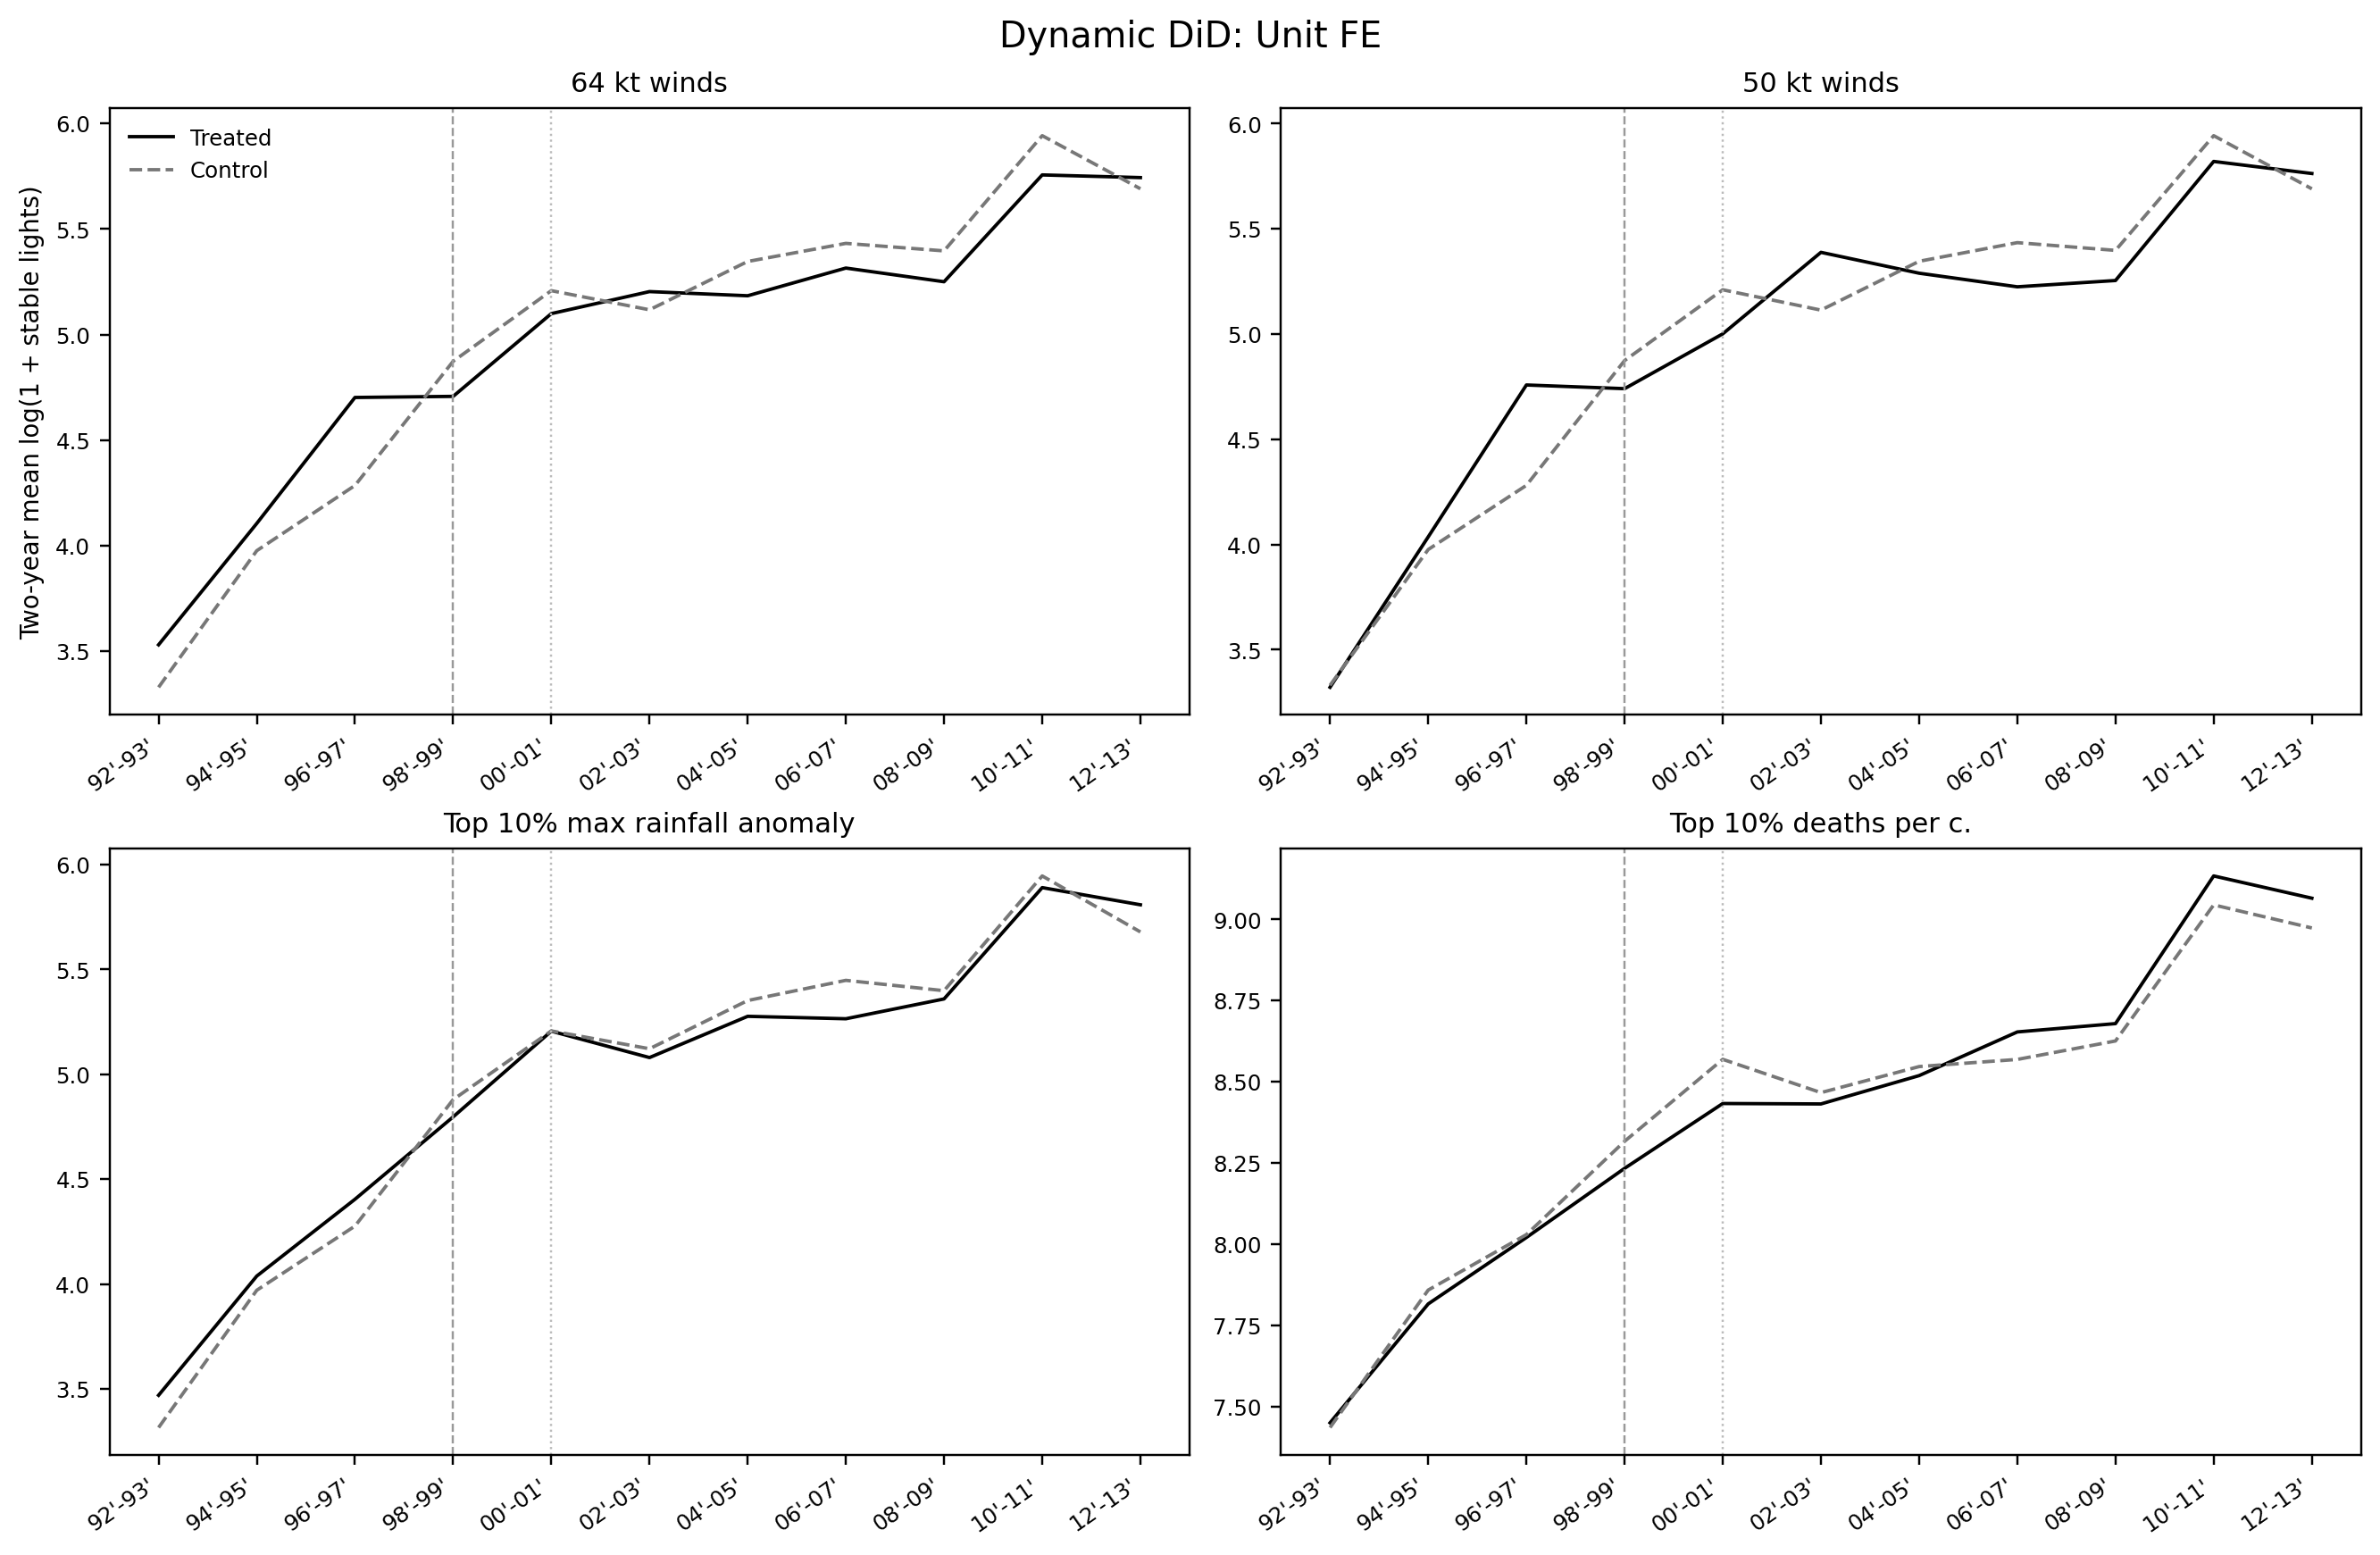
\includegraphics[width=0.94\linewidth]{Paper_Figures/legacy/main_results/figures/dynamic_did/no_year_fe/fig_four_treatments_no34.png}
\widefigurenotes{The panels plot treated and comparison-group means of $\log(1+\text{stable lights})$ after removing time-invariant unit differences. Calendar-year fixed effects and the pre-Mitch median luminosity filter are not applied.}
\end{figure}

% P23: Results, preferred event-study display
\begin{figure}[p]
\centering
\caption{\label{fig:event-ebtrk-thresholds}Two-year coefficient estimates with year fixed effects and the NTL filter}
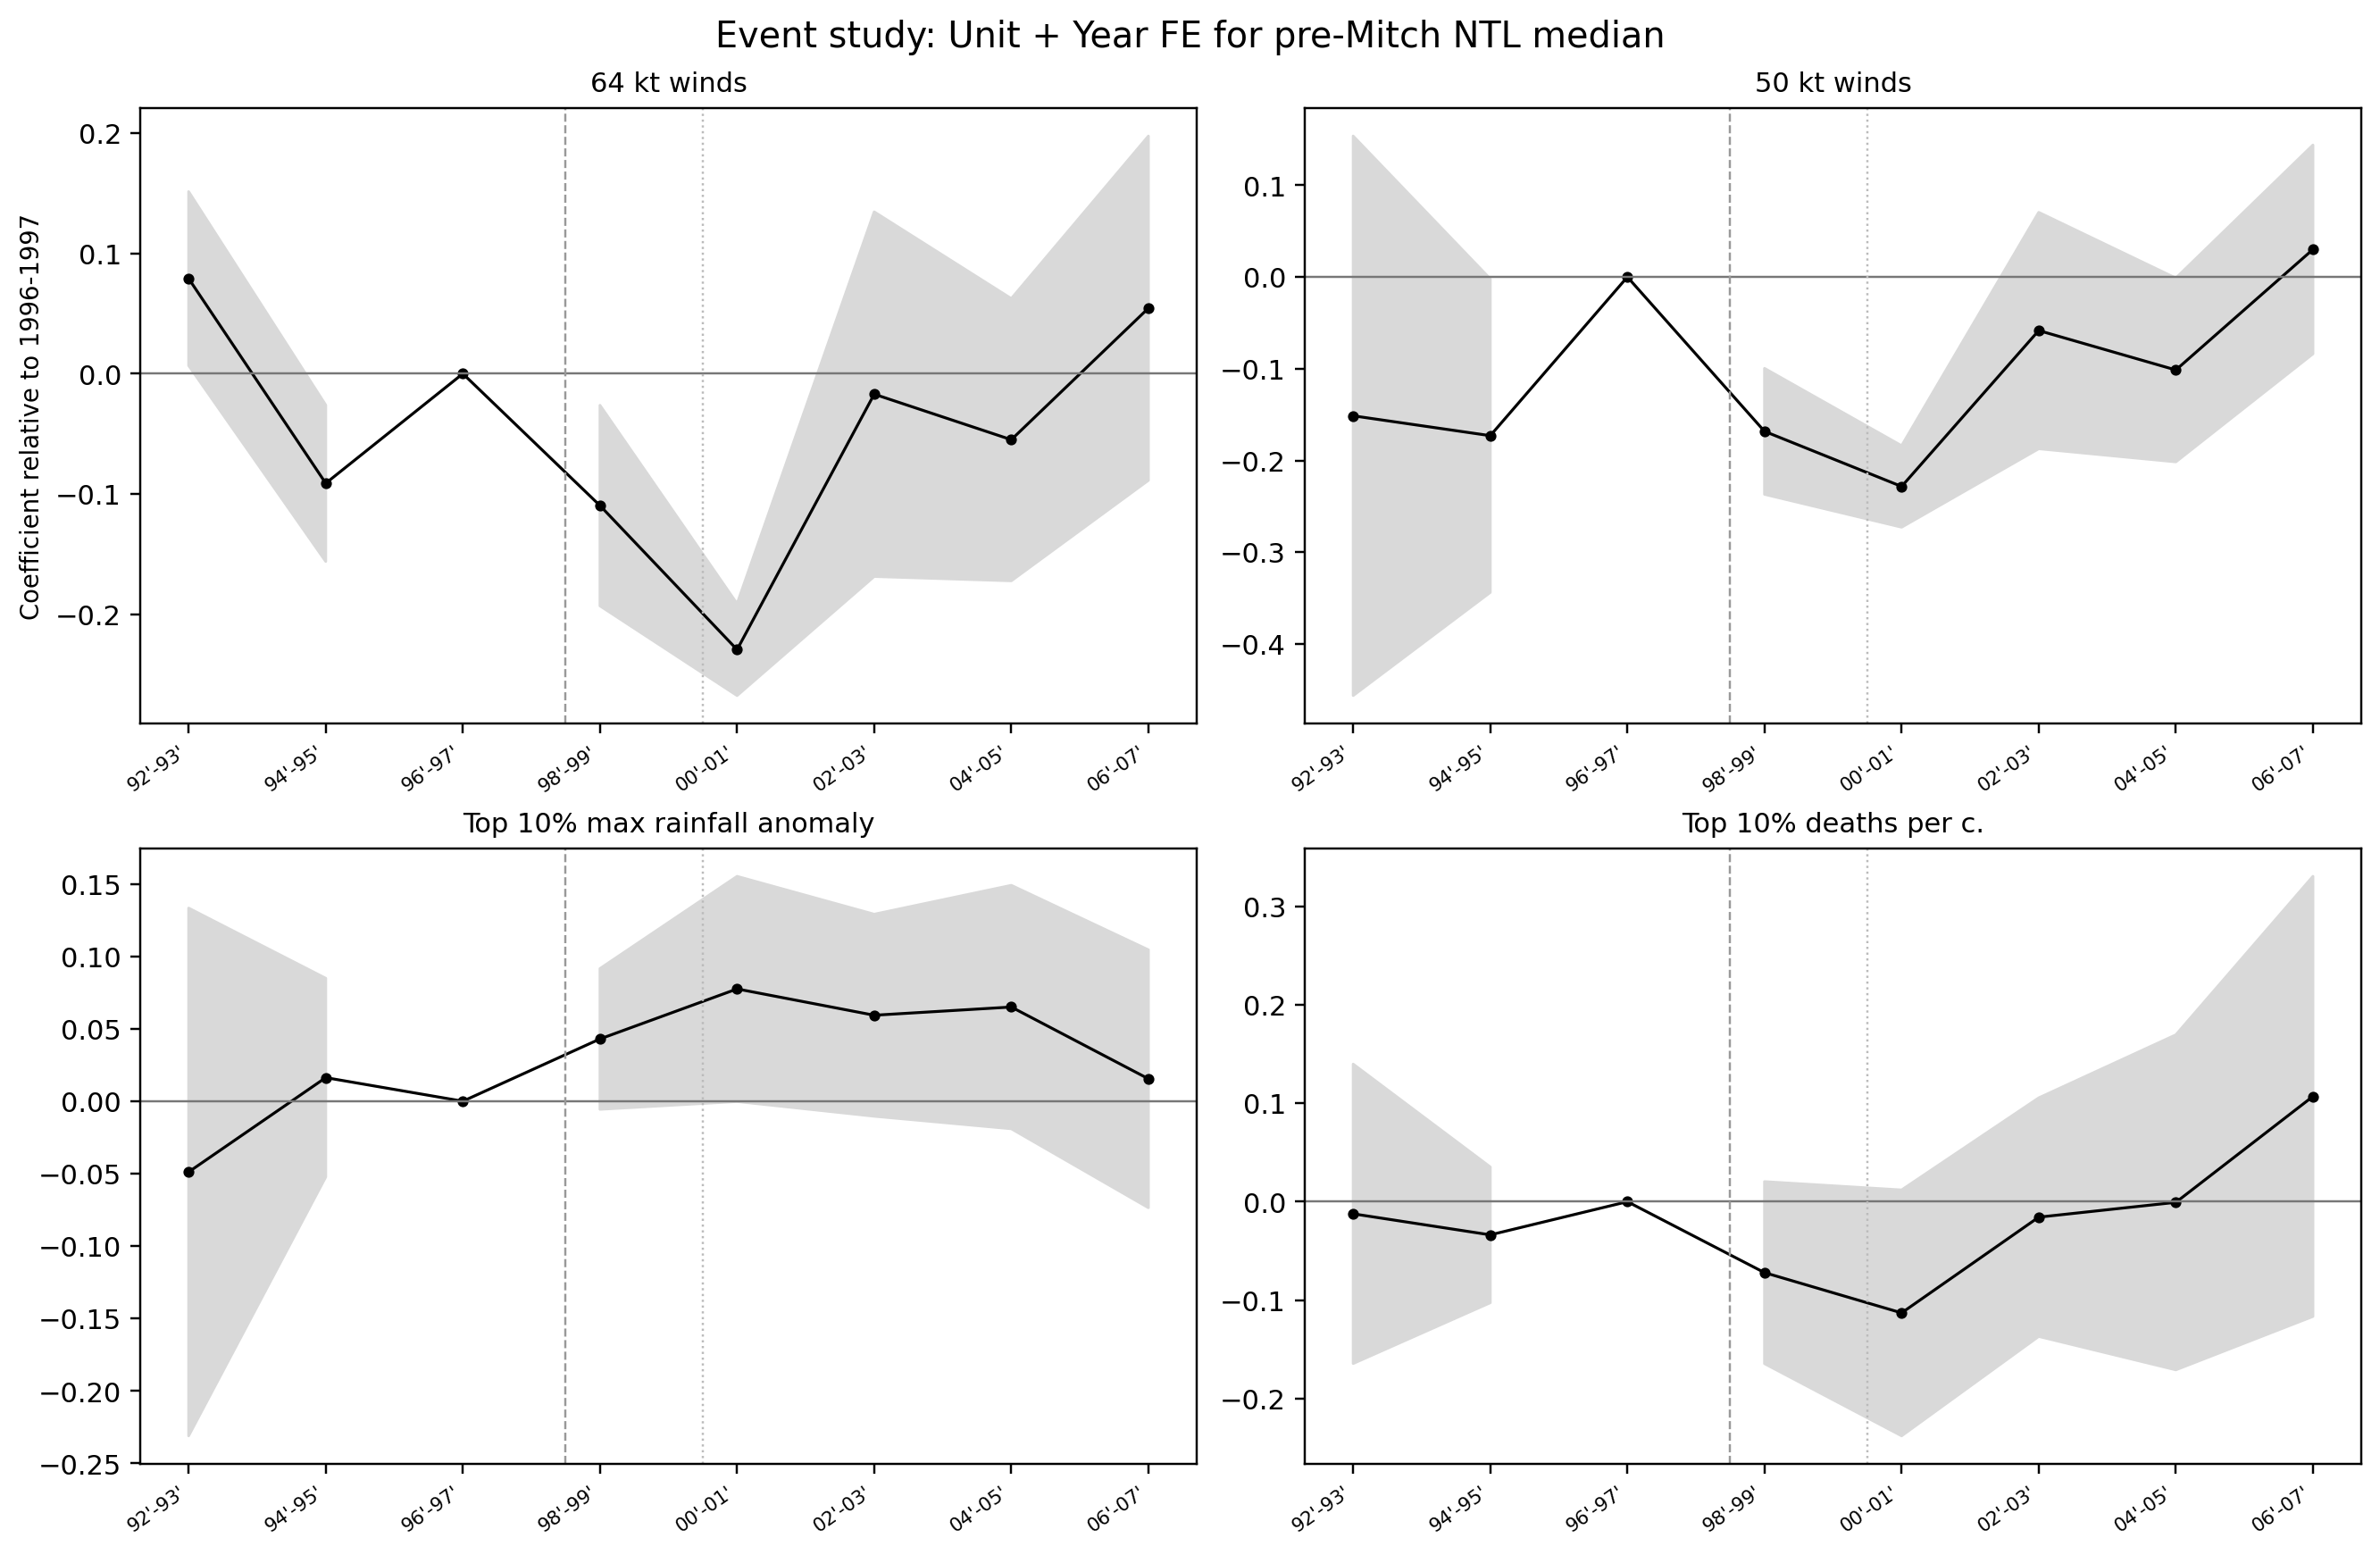
\includegraphics[width=0.90\linewidth]{Paper_Figures/main_results/figures/event_study/year_fe_ntl_filter/fig_four_treatments_no34.png}
\widefigurenotes{The figure plots two-year treatment-period coefficients from the Unit + Year FE specification restricted to units at or above the pre-Mitch median luminosity of 101.79. The omitted period is 1996--1997 and shaded bands show approximate 95 percent confidence intervals.}
\end{figure}

% P24: Results, main regression table
\begin{table}[htbp]
\centering
\caption{\label{tab:ebtrk-binary-reg}Two-year coefficients for main treatment definitions}
\begingroup
\scriptsize
\setlength{\tabcolsep}{3pt}
\resizebox{\linewidth}{!}{%
\begin{tabular}{llrrrrrrrrr}
\toprule
Treatment & Specification & 92'-93' & 94'-95' & 96'-97' & 98'-99' & 00'-01' & 02'-03' & 04'-05' & 06'-07' & 08'-09'$\ldots$ \\
\midrule
64 kt & Unit + Year FE & \begin{tabular}{@{}c@{}}-0.216\\{\scriptsize (0.314)}\end{tabular} & \begin{tabular}{@{}c@{}}-0.288\\{\scriptsize (0.180)}\end{tabular} & ref. & \cellcolor{gray!11}\begin{tabular}{@{}c@{}}-0.583\\{\scriptsize (0.559)}\end{tabular} & \cellcolor{gray!11}\begin{tabular}{@{}c@{}}-0.526\\{\scriptsize (0.550)}\end{tabular} & \cellcolor{gray!11}\begin{tabular}{@{}c@{}}-0.331\\{\scriptsize (0.572)}\end{tabular} & \cellcolor{gray!11}\begin{tabular}{@{}c@{}}-0.579\\{\scriptsize (0.530)}\end{tabular} & \cellcolor{gray!11}\begin{tabular}{@{}c@{}}-0.534\\{\scriptsize (0.546)}\end{tabular} & \cellcolor{gray!11}\begin{tabular}{@{}c@{}}-0.563\\{\scriptsize (0.569)}\end{tabular} \\
 & \begin{tabular}{@{}l@{}}Unit + Year FE\\for pre-Mitch NTL median\end{tabular} & \begin{tabular}{@{}c@{}}0.079**\\{\scriptsize (0.037)}\end{tabular} & \begin{tabular}{@{}c@{}}-0.091***\\{\scriptsize (0.033)}\end{tabular} & ref. & \cellcolor{gray!39}\begin{tabular}{@{}c@{}}-0.110***\\{\scriptsize (0.042)}\end{tabular} & \cellcolor{gray!39}\begin{tabular}{@{}c@{}}-0.229***\\{\scriptsize (0.019)}\end{tabular} & \cellcolor{gray!11}\begin{tabular}{@{}c@{}}-0.017\\{\scriptsize (0.077)}\end{tabular} & \cellcolor{gray!11}\begin{tabular}{@{}c@{}}-0.055\\{\scriptsize (0.060)}\end{tabular} & \begin{tabular}{@{}c@{}}0.054\\{\scriptsize (0.073)}\end{tabular} & \begin{tabular}{@{}c@{}}0.002\\{\scriptsize (0.024)}\end{tabular} \\
\addlinespace
50 kt & Unit + Year FE & \begin{tabular}{@{}c@{}}-0.486\\{\scriptsize (0.304)}\end{tabular} & \begin{tabular}{@{}c@{}}-0.417**\\{\scriptsize (0.166)}\end{tabular} & ref. & \cellcolor{gray!21}\begin{tabular}{@{}c@{}}-0.610*\\{\scriptsize (0.332)}\end{tabular} & \cellcolor{gray!30}\begin{tabular}{@{}c@{}}-0.686**\\{\scriptsize (0.327)}\end{tabular} & \cellcolor{gray!11}\begin{tabular}{@{}c@{}}-0.202\\{\scriptsize (0.356)}\end{tabular} & \cellcolor{gray!21}\begin{tabular}{@{}c@{}}-0.534*\\{\scriptsize (0.321)}\end{tabular} & \cellcolor{gray!30}\begin{tabular}{@{}c@{}}-0.687**\\{\scriptsize (0.331)}\end{tabular} & \cellcolor{gray!21}\begin{tabular}{@{}c@{}}-0.620*\\{\scriptsize (0.323)}\end{tabular} \\
 & \begin{tabular}{@{}l@{}}Unit + Year FE\\for pre-Mitch NTL median\end{tabular} & \begin{tabular}{@{}c@{}}-0.151\\{\scriptsize (0.156)}\end{tabular} & \begin{tabular}{@{}c@{}}-0.173**\\{\scriptsize (0.087)}\end{tabular} & ref. & \cellcolor{gray!39}\begin{tabular}{@{}c@{}}-0.168***\\{\scriptsize (0.035)}\end{tabular} & \cellcolor{gray!39}\begin{tabular}{@{}c@{}}-0.228***\\{\scriptsize (0.023)}\end{tabular} & \cellcolor{gray!11}\begin{tabular}{@{}c@{}}-0.058\\{\scriptsize (0.066)}\end{tabular} & \cellcolor{gray!30}\begin{tabular}{@{}c@{}}-0.101**\\{\scriptsize (0.051)}\end{tabular} & \begin{tabular}{@{}c@{}}0.030\\{\scriptsize (0.058)}\end{tabular} & \begin{tabular}{@{}c@{}}0.015\\{\scriptsize (0.028)}\end{tabular} \\
\addlinespace
Top 10\% rain & Unit + Year FE & \begin{tabular}{@{}c@{}}0.026\\{\scriptsize (0.114)}\end{tabular} & \begin{tabular}{@{}c@{}}-0.060\\{\scriptsize (0.078)}\end{tabular} & ref. & \cellcolor{gray!39}\begin{tabular}{@{}c@{}}-0.210***\\{\scriptsize (0.055)}\end{tabular} & \cellcolor{gray!11}\begin{tabular}{@{}c@{}}-0.129\\{\scriptsize (0.096)}\end{tabular} & \cellcolor{gray!21}\begin{tabular}{@{}c@{}}-0.170*\\{\scriptsize (0.091)}\end{tabular} & \cellcolor{gray!21}\begin{tabular}{@{}c@{}}-0.203*\\{\scriptsize (0.115)}\end{tabular} & \cellcolor{gray!39}\begin{tabular}{@{}c@{}}-0.311***\\{\scriptsize (0.116)}\end{tabular} & \cellcolor{gray!11}\begin{tabular}{@{}c@{}}-0.167\\{\scriptsize (0.127)}\end{tabular} \\
 & \begin{tabular}{@{}l@{}}Unit + Year FE\\for pre-Mitch NTL median\end{tabular} & \begin{tabular}{@{}c@{}}-0.049\\{\scriptsize (0.093)}\end{tabular} & \begin{tabular}{@{}c@{}}0.016\\{\scriptsize (0.035)}\end{tabular} & ref. & \begin{tabular}{@{}c@{}}0.043*\\{\scriptsize (0.025)}\end{tabular} & \begin{tabular}{@{}c@{}}0.077*\\{\scriptsize (0.040)}\end{tabular} & \begin{tabular}{@{}c@{}}0.059*\\{\scriptsize (0.036)}\end{tabular} & \begin{tabular}{@{}c@{}}0.065\\{\scriptsize (0.043)}\end{tabular} & \begin{tabular}{@{}c@{}}0.015\\{\scriptsize (0.045)}\end{tabular} & \cellcolor{gray!11}\begin{tabular}{@{}c@{}}-0.021\\{\scriptsize (0.042)}\end{tabular} \\
\addlinespace
Top 10\% deaths per c. & Unit + Year FE & \begin{tabular}{@{}c@{}}0.023\\{\scriptsize (0.085)}\end{tabular} & \begin{tabular}{@{}c@{}}-0.034\\{\scriptsize (0.035)}\end{tabular} & ref. & \cellcolor{gray!11}\begin{tabular}{@{}c@{}}-0.074\\{\scriptsize (0.047)}\end{tabular} & \cellcolor{gray!21}\begin{tabular}{@{}c@{}}-0.127*\\{\scriptsize (0.065)}\end{tabular} & \cellcolor{gray!11}\begin{tabular}{@{}c@{}}-0.026\\{\scriptsize (0.062)}\end{tabular} & \cellcolor{gray!11}\begin{tabular}{@{}c@{}}-0.019\\{\scriptsize (0.088)}\end{tabular} & \begin{tabular}{@{}c@{}}0.094\\{\scriptsize (0.114)}\end{tabular} & \begin{tabular}{@{}c@{}}0.062\\{\scriptsize (0.099)}\end{tabular} \\
 & \begin{tabular}{@{}l@{}}Unit + Year FE\\for pre-Mitch NTL median\end{tabular} & \begin{tabular}{@{}c@{}}-0.012\\{\scriptsize (0.078)}\end{tabular} & \begin{tabular}{@{}c@{}}-0.034\\{\scriptsize (0.035)}\end{tabular} & ref. & \cellcolor{gray!11}\begin{tabular}{@{}c@{}}-0.072\\{\scriptsize (0.047)}\end{tabular} & \cellcolor{gray!21}\begin{tabular}{@{}c@{}}-0.113*\\{\scriptsize (0.064)}\end{tabular} & \cellcolor{gray!11}\begin{tabular}{@{}c@{}}-0.016\\{\scriptsize (0.062)}\end{tabular} & \cellcolor{gray!11}\begin{tabular}{@{}c@{}}-0.001\\{\scriptsize (0.087)}\end{tabular} & \begin{tabular}{@{}c@{}}0.107\\{\scriptsize (0.114)}\end{tabular} & \begin{tabular}{@{}c@{}}0.080\\{\scriptsize (0.098)}\end{tabular} \\
\bottomrule
\end{tabular}

}
\endgroup
\tablenotes{The outcome is log(1 + DMSP-OLS stable lights). Rows report specifications with unit and year fixed effects, with and without the pre-Mitch median luminosity filter. Columns report selected two-year treatment-period coefficients relative to 1996--1997, the omitted reference period; unreported later bins through 2012--2013 are included in estimation. Standard errors are clustered by the estimation unit.}
\end{table}

% P25: Results, delayed relative divergence
Consistently across specifications, the largest relative loss occurs over the second period rather than immediately after landfall. Deaths-per-capita, for example, shows its largest and only conventionally statistically significant loss during the 2000--2001 period whether luminosity filtered or not. As the annualized appendix specifications show the same pattern across specifications, the pattern is unlikely to be only an artifact of the two-year binning which makes 98-99' a mix of pre- and post-Mitch years. In the appendix 1999 coefficients, a fully post-Mitch year, are consistently smaller and less significant than 2000 coefficient. A more plausible interpretation is a delayed relative divergence. Treated municipalities did not continue falling, but plated below their previous path, while comparison municipalities continued growing; the difference-in-differences gap therefore widened into 2000 before closing by 2002--2003. This would imply a quick subsequent rebound consistent with Solow-style recovery interpretations where the fastest capital replacements are possible after destruction.

\subsection{Liberal Income Translation and Census Robustness Check}

% P26: Results, income translation and resilience calculation
While the nighttime-light losses cannot be directly translated into an income amount for treated municipalities, they can provide an order-of-magnitude input for local planning. This is contingent on the accuracy of elasticites used for translation. Ishizawa, Miranda, and Zhang report elasticities of real GDP with respect to lights in Central America ranging from 0.1581 to 0.2326. Applying those elasticities to the filtered 50-knot estimates implies income-equivalent losses of approximately 2.45--3.60 percent in 1998--1999 and 3.23--4.75 percent in 2000--2001. For every \$1 million in annual local output exposed to a comparable 50-knot shock, measured in 2026 dollars, this corresponds to roughly \$114,000--\$167,000 in lost income-equivalent activity across four years. If a targeted \$50,000 resilience investment prevented 40 percent of those losses, avoided income losses alone could be about \$45,000--\$67,000, before counting avoided deaths, displacement, and reconstruction costs. 

% P27: Results, census description of treated places
Resilience investments would then have to be grounded in local conditions, which Table \ref{tab:ipums-resilience} describes 
in a limited fashion using harmonized Honduran census groups. These groups combine legal municipalities for ease of the census process, so some contain both treated and untreated municipalities, but most groups were hit together. Between 1988 and 2013 treated municipality groups improved substantially in electricity, sanitation, and masonry, yet exposure-relevant vulnerability remained. In particular, 83.3 percent of households had sheet-metal roofs in 2013. Though plausible improvements from sun-dried mud or palm fronds, poorly fastened panels can lift under hurricane winds, exposing occupants and their possessions to wind-driven rain. The quality of the masonry walls reported should also be examined. 

\begin{table}[p]
\centering
\caption{\label{tab:ipums-resilience}Population, education, and dwelling conditions in Honduran 50-knot census groups}
\begingroup
\scriptsize
\setlength{\tabcolsep}{3pt}
\textbf{Panel A. Population and adult education in census years}
\par\smallskip
\resizebox{\linewidth}{!}{%
\begin{tabular}{lcrrrrrr}
\toprule
 & & \multicolumn{3}{c}{Population (thousands)} & \multicolumn{3}{c}{Mean school years, age 25+} \\
\cmidrule(lr){3-5}\cmidrule(lr){6-8}
IPUMS geography & 50-kt coverage & 1988 & 2001 & 2013 & 1988 & 2001 & 2013 \\
\midrule
Colon group: Balfate--Iriona & 7/7 & 66.5 & 112.2 & 148.9 & 2.5 & 3.5 & 4.7 \\
Colon group: Saba--Tocoa & 3/3 & 78.0 & 107.3 & 163.8 & 2.7 & 4.1 & 5.3 \\
Bay Islands group & 3/4 & 21.5 & 31.2 & 63.7 & 4.6 & 6.2 & 7.0 \\
Olancho group: Gualaco--San Esteban & 2/2 & 24.6 & 37.7 & 47.2 & 1.7 & 3.0 & 4.2 \\
Honduras &  & 4,239.7 & 6,086.2 & 8,303.1 & 3.4 & 4.8 & 5.7 \\
Gracias a Dios group* & 1/6 & 33.2 & 57.5 & 89.5 & 2.7 & 3.9 & 5.0 \\
\bottomrule
\end{tabular}%
}
\par\medskip
\textbf{Panel B. Household-weighted dwelling characteristics}
\par\smallskip
\resizebox{\linewidth}{!}{%
\begin{tabular}{lrrrrrrrrrrrr}
\toprule
 & \multicolumn{3}{c}{1974} & \multicolumn{3}{c}{1988} & \multicolumn{3}{c}{2001} & \multicolumn{3}{c}{2013} \\
\cmidrule(lr){2-4}\cmidrule(lr){5-7}\cmidrule(lr){8-10}\cmidrule(lr){11-13}
Characteristic (\% of households) & Treated & Honduras & Diff. & Treated & Honduras & Diff. & Treated & Honduras & Diff. & Treated & Honduras & Diff. \\
\midrule
Electricity & -- & -- & -- & 23.2 & 39.6 & -16.5 & 48.6 & 60.2 & -11.6 & 78.2 & 80.8 & -2.6 \\
Sewer or septic & -- & -- & -- & 11.2 & 26.7 & -15.5 & 41.9 & 50.8 & -8.9 & 74.8 & 68.7 & +6.1 \\
Masonry wall & -- & -- & -- & 18.2 & 24.6 & -6.4 & 55.4 & 46.6 & +8.8 & 68.9 & 53.8 & +15.2 \\
Sheet-metal roof & -- & -- & -- & 41.6 & 38.4 & +3.2 & 61.1 & 47.9 & +13.2 & 83.3 & 63.7 & +19.5 \\
Refrigerator & -- & -- & -- & 12.2 & 19.3 & -7.1 & 28.2 & 34.5 & -6.3 & 57.5 & 59.4 & -1.9 \\
Television & -- & -- & -- & 5.5 & 29.3 & -23.8 & 30.3 & 47.9 & -17.7 & 61.4 & 67.1 & -5.7 \\
\bottomrule
\end{tabular}%
}

\endgroup
\tablenotes{Panel A reports weighted population and mean years of schooling among adults age 25 and older. The coverage column gives treated legal municipalities over all municipalities in each harmonized IPUMS group and is blank for Honduras. Panel B compares the three cleanly treated groups with Honduras and reports the treated-minus-Honduras difference. The 1974 census is shown because it would provide a valuable second pre-Mitch observation, but the requested household variables are not reported in that sample. The asterisk marks the Gracias a Dios group, which is not used in the DiDs discussed in P29 because only one of its six municipalities is treated; the mixed Bay Islands group is also excluded. Source: IPUMS International and author's calculations \parencite{ipumsinternational2025}.}
\end{table}

% P28: Results, census normal-goods robustness design
The dwelling characteristics named in Table \ref{tab:ipums-resilience} can also be used a simple robustness checks for the temporary nightlight loss found in this paper. Whether households have refrigerators or televisions in particular provide a straightforward check as normal goods like nightlights. 

 If Mitch caused a persistent income loss that the nighttime-light recovery missed, ownership in cleanly treated groups should fall relative to controls by 2001 when compared with the 1988 gap. This test is limited by census frequency and variable availability: although Honduras has a 1974 census, household assets are reported only starting from 1988 leaving only one pre-Mitch benchmark. Even worse, these assets represent some of the strongest income proxies in census data, the others being only education or worker type\footnote{A preliminary cohort-by-year education exercise found that people born in cleanly treated groups who were ages 6--11 at Mitch completed 0.36 fewer years of schooling relative to older cohorts (SE 0.16). However, specification produced large nonzero 1961 and 1974 treatment interactions relative to 1988 (0.46 and 0.61), weakening the parallel-trends case.}

% P29: Results, census robustness findings
Contributing to the paper robustness, the census DiD estimates are largely null results and do not corroborate a persistent negative normal-goods effect. Relative to 1988, the 2001 coefficients are 3.1 percentage points for refrigerator ownership (SE 4.8) and 9.1 points for television ownership (SE 7.3); the 2013 estimates are 6.7 (SE 7.5) and 20.8 (SE 8.8), respectively. Figure \ref{fig:appendix-normal-goods} and Table \ref{tab:normal-goods} in the appendix report these estimates with Gracias a Dios and the mixed Bay Islands group excluded. The null or positive estimates are consistent with recovery by the 2001 census. The census' null results confirm that NTL data can reveal a multi-year suppression of that local census in countries with poor data infrastructure conceal. They strengthen the the validity of a four-year recovery path, which would have failed outside available census years, while demonstrating that satellite-derived measures can capture high-frequency disaster dynamics that would have been lost otherwise.

\clearpage
\section{Discussion}
% P30: Discussion, what the paper measures
\begin{quote}
\centering
``In 72 hours we lost what took as much as 50 years to build.''\\
\hfill Carlos Flores Facussé, November 1998 \parencite{collier1998mitch}
\end{quote}
It is worth concluding by returning to the quotation, ingrained in many Hondurans' minds, from which this paper was born. The paper estimated only part of the loss through the evolution of municipality-level nighttime lights after physically reconstructed Mitch exposure. The preferred wind specifications identified a 10--20 percent relative luminosity loss during the first four post-storm years, followed by a closing of the treated-control gap. The census checks likewise provide no evidence of a persistent negative refrigerator or television effect by 2001, but to Facusse's credit neither source measured destruction in full.
% P31: Discussion, flood measurement options

Wind swaths offer a compratively transparent physical assignment with infrastructure damage thresholds that has attracted economics. Flooding, the clearest damage omission in this paper, does not. In its simplest terms, flooding is when the the lands input of perceptions becomes greater than its capability to retain or output. From this it becomes a mind-bending mix of landscapes, atmospheres and built geography and timescapes, past rain and current retention levels. The failure of the top-decile CHIRPS anomaly specification in this paper points difficulty of measuring it. Flooding interacts with the socioeconomic as well, there is a reason the poorest houses in Tegucigalpa, a frequently flooded and mountain surrounded capital, are along the Echolocate River. They were homes that were devastated after Mitch as shown in Figure \ref{fig}. Yet, weather because the city wide effects remained small or because flooding was not properly measured none of the treatment specifications used here counted the capital's municipality as treated. Furthermore, only CHIRPS continued Nicaraguan municpalities as treated though Mitch's devstation led them to be granted temporary protected status, and as Figure x showed it received the most rainfall anomally, particularly around the golf of Fonseca.

\begin{figure}[htbp]
\centering
\caption{\label{fig}Hurricane Mitch damage in Tegucigalpa}
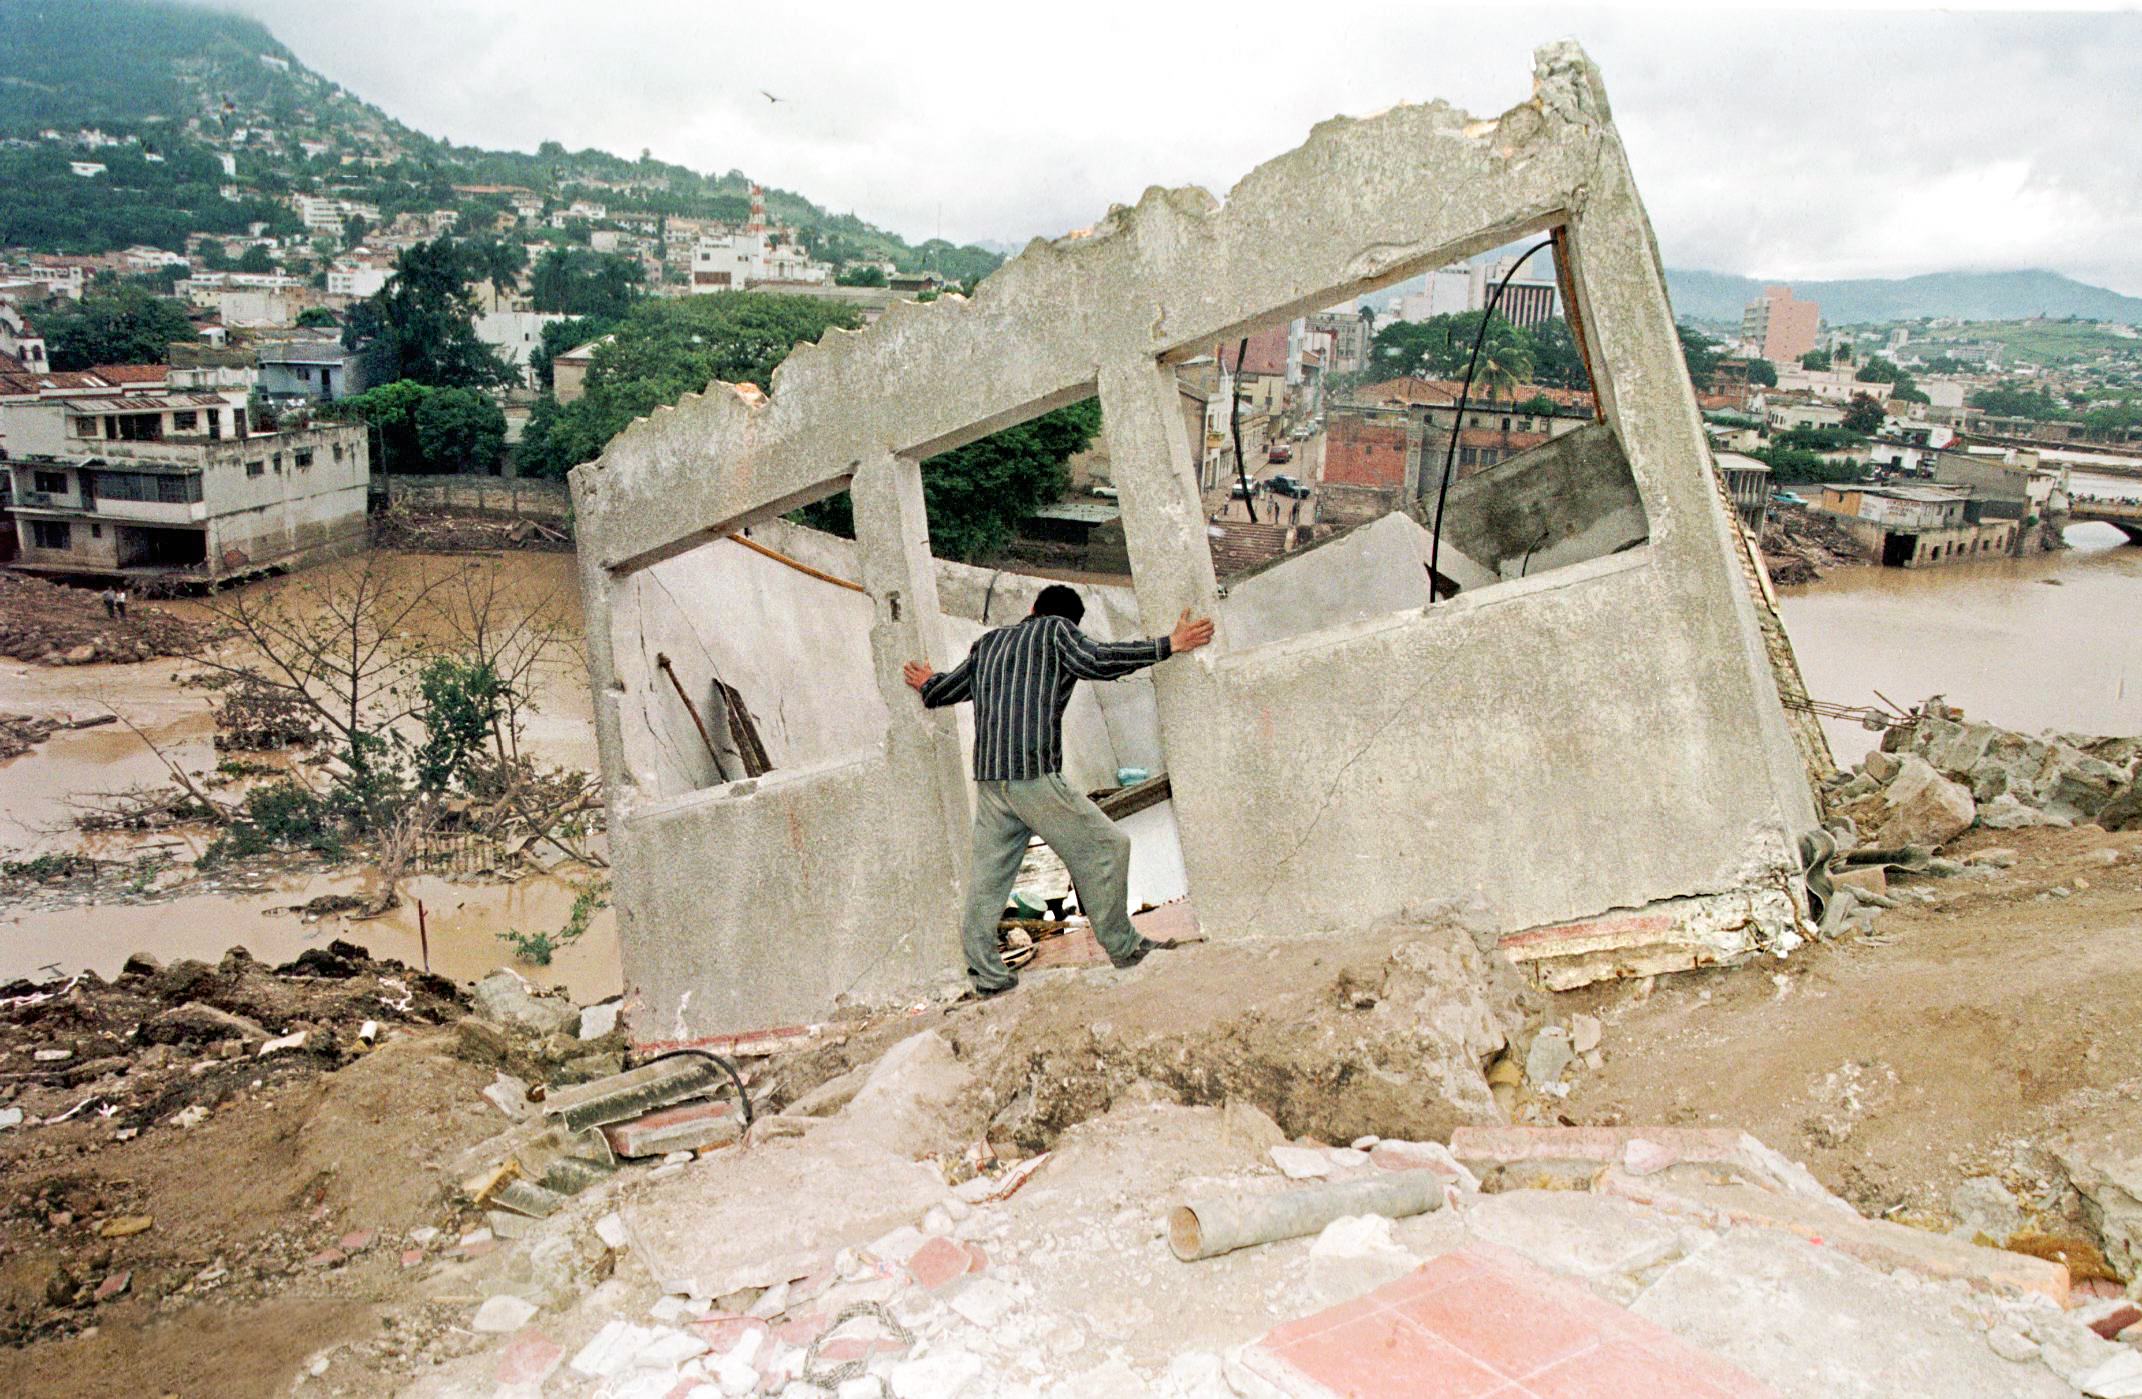
\includegraphics[width=0.88\linewidth]{Paper_Figures/presentation/Tegucigalpa.jpg}
\figurenotes{Damage in Tegucigalpa was concentrated along the Choluteca River. \textbf{The figure illustrates a form of Mitch damage not captured by the strict wind-treatment definitions. Add original image source before submission if this image is not author-owned.}}
\end{figure}

Flooding which is the meeting point of atmosphere and land and the meeting of temporaries as well.

lands capability to retain or output water becomes less than 

Flooding is the clearest omission. Wind swaths offer a comparatively transparent physical assignment with infrastructure damage thresholds, they have a simplicity which flooding which damaged large parts of Central America does not. They have been proffered by economists. The failure of the top-decile CHIRPS anomaly specification in this paper points to the difficulties in measuring flooding which is inherently a cross-geographical and cross-temporal phenomenon. The meeting point of the atmosphere with the built and natural geography, rivers, mountains which may channel water, or draining that is improperly built. There is reason the poorest houses in the frequently flooded  and mountain surrounded Tegucigalpa are along the Choluteca river where property prices are low and flood risks high. None of the treatment speficiations in this paper counted Tegucigalpa as trated, as a whole it may not be, but for many like in the Figure below there were devasting effects. Timelines mattered, if in the previous month the choluteca river recieved more rain than usual the consquences would be greater. 

\vspace{0.25cm}
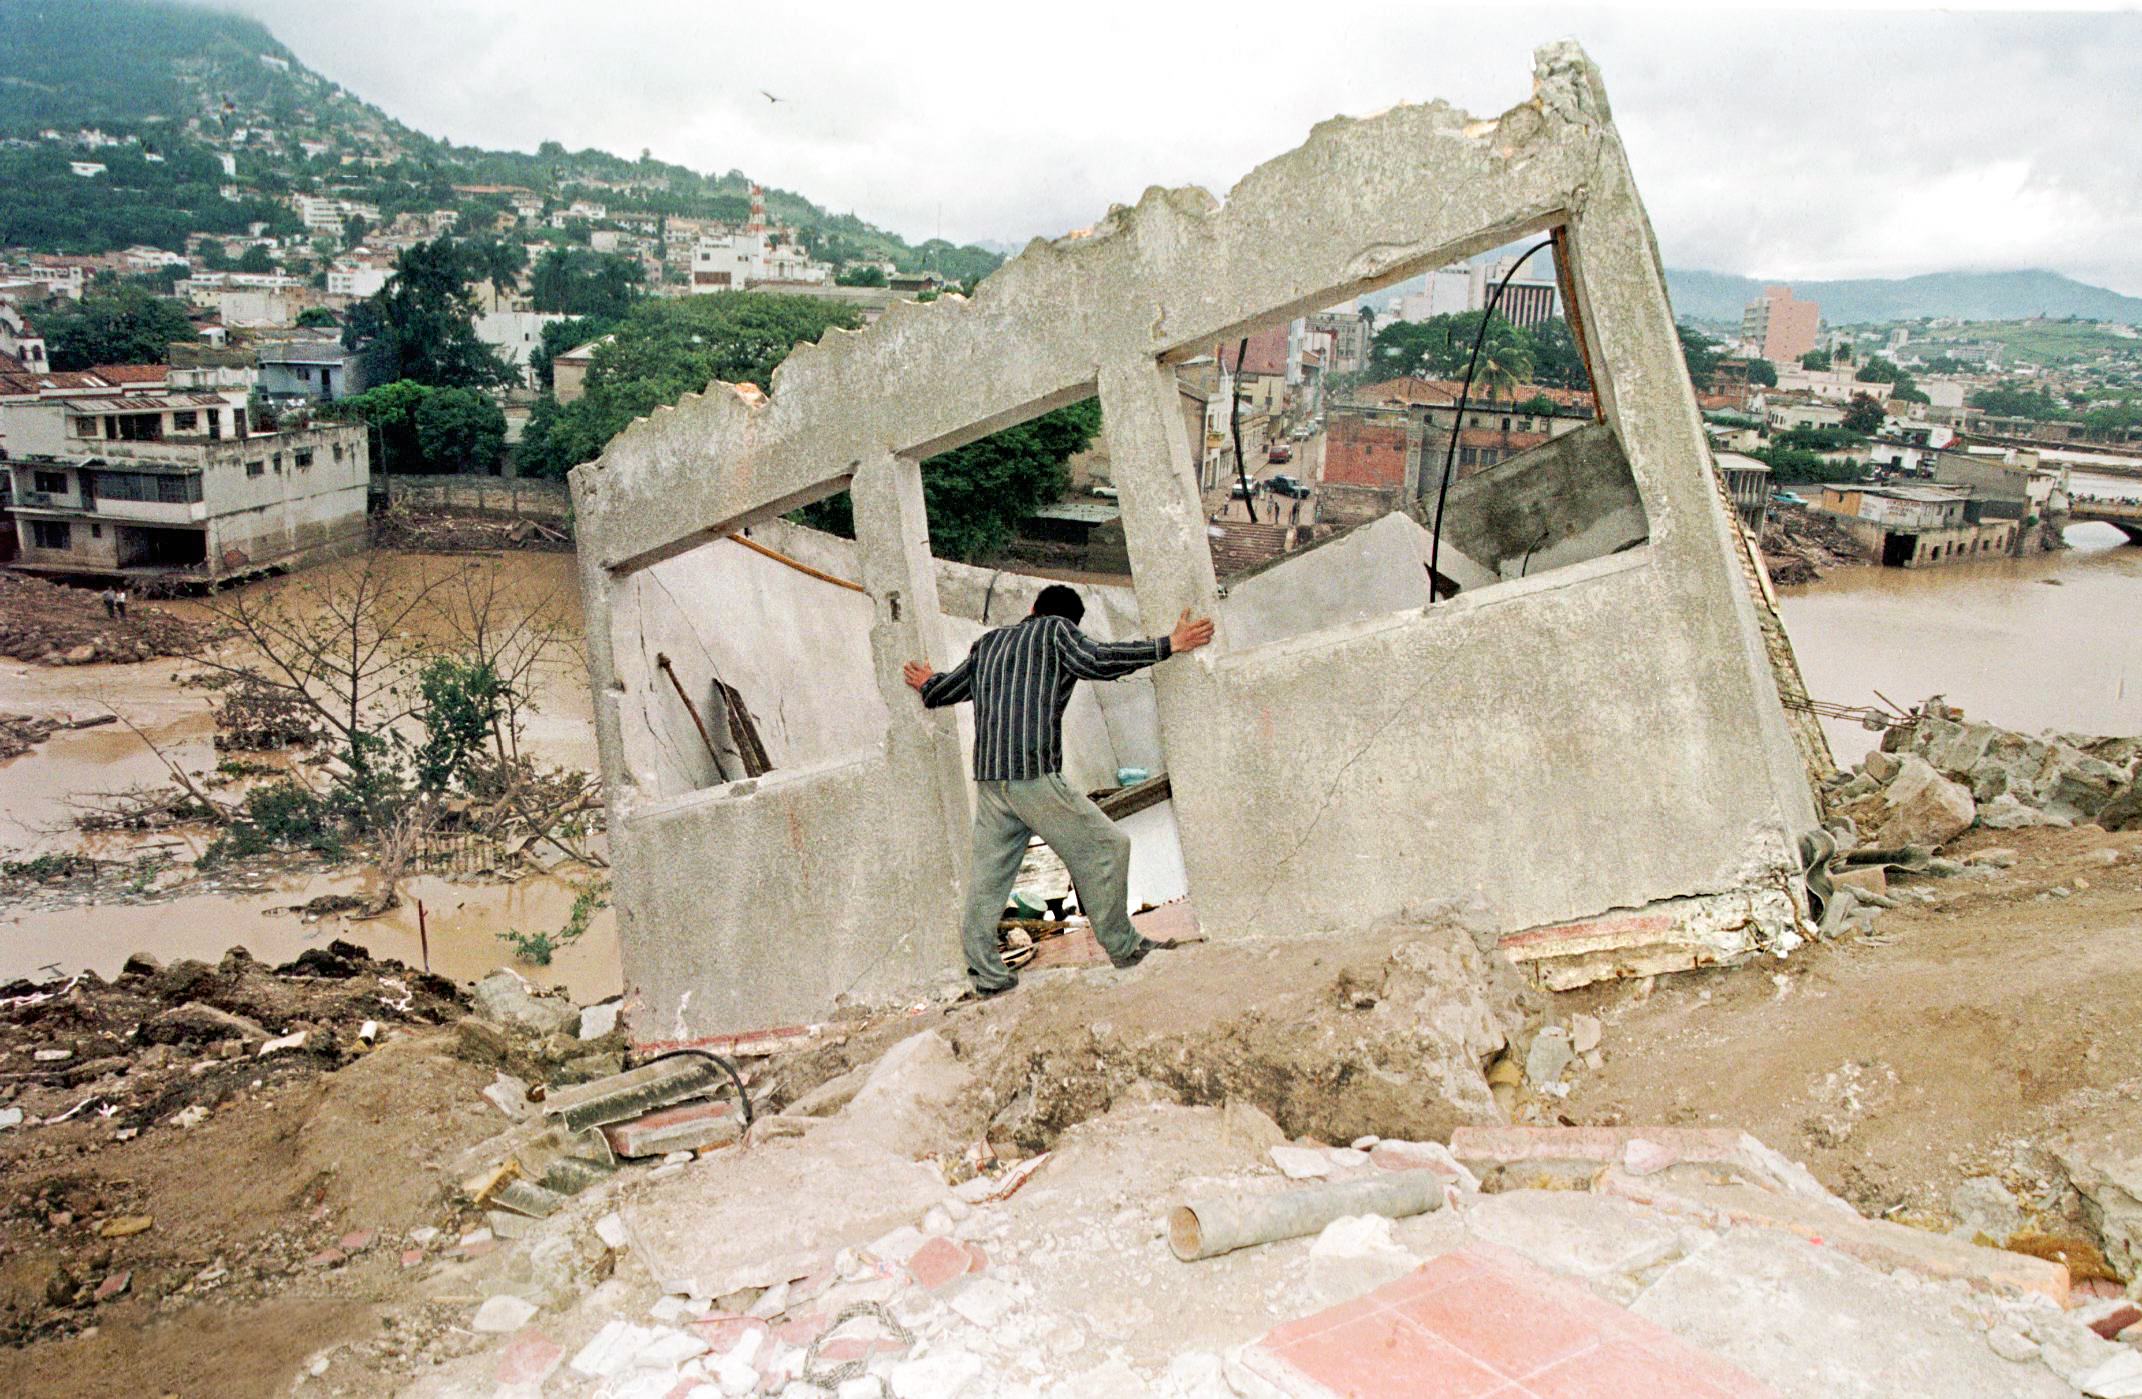
\includegraphics[width=\linewidth,height=0.34\textheight,keepaspectratio]{Paper_Figures/presentation/Tegucigalpa.jpg}

{\scriptsize Damage in Tegucigalpa, concentrated along river}

What would a specification look like that could consider the natural and built geography? Ideally... Then describe WRI aquedect floods and the pros anc cons this would face

Wind swaths offer a comparatively transparent physical assignment, while the top-decile CHIRPS anomaly does not model how rainfall interacts with rivers, slopes, soils, drainage, defenses, and settlement. A second is WRI's Aqueduct Floods, which is open and reproducible and links riverine and coastal hazard to population, assets, and protection, but is coarser and less suited to neighborhood-scale flash flooding and landslides \parencite{wri2020aqueductfloods}. The ideal extension would reconstruct Mitch-specific runoff and flood depth from its rainfall field and 1998 terrain, river, land-cover, drainage, and defense conditions, then overlay contemporaneous population, housing, and infrastructure.

% P32: Discussion, recovery and conclusion
Part of the loss however was temporary, part of the loss that an account of flooding might also find may be temporary as well. The northern Honduran municipalitie. That result was not the simple story I expected, and in some ways Facusse was wrong. Queue the music, this would be the part of the paper where I remember those 9,000 that died, and those 9,000 that dissapeared. Their loss is without a douhbt incomensurable. But, it is also within economics profane beauty to move with rigor and evidence beyond simplistic explanations and shocking images. Though the loss of Mitch was incomenasurable, though I had though it set us on irreperable path, unless there is evidence that can point otherwise I must also believe this may not be the case. That the reason for our backwardness may well lie in insert: boring economcis thing related to Honduras, insert: boring economics related to Honduras. God knows they are more boring, less striking than the videos of Hurricanes that can be found. But when aggregated over millions, when show in significanes there force may well be stronger than a Hurricane. 

\clearpage

\appendix

\section{Expanded Summary Statistics}
\label{app:expanded-summary}
\begin{table}[p]
\centering
\caption{\label{tab:appendix-expanded-summary}Expanded summary statistics}
\begin{minipage}{\linewidth}
\centering
\scriptsize
\setlength{\tabcolsep}{3pt}
\textbf{Panel A. Dependent nighttime-lights panel}\par\vspace{0.25em}
\resizebox{\linewidth}{!}{%
\begin{tabular}{lllrrrrrr}
\toprule
Outcome & Source & Sample & Mean & SD & P10 & P50 & P90 & Obs \\
\midrule
Stable lights, all years & DMSP-OLS & All retained municipalities & 587.4 & 1,368 & 0.361373 & 218.0 & 1,359 & 21,912 \\
Stable lights, 1998 & DMSP-OLS & All retained municipalities & 498.2 & 1,242 & 0 & 185.9 & 1,126 & 996 \\
log(1 + stable lights), all years & DMSP-OLS & All retained municipalities & 4.963 & 2.162 & 0.308493 & 5.389 & 7.216 & 21,912 \\
Stable lights, all years & DMSP-OLS & Pre-Mitch NTL at or above median (101.79) & 1,053 & 1,811 & 173.3 & 552.1 & 2,182 & 10,956 \\
Stable lights, 1998 & DMSP-OLS & Pre-Mitch NTL at or above median (101.79) & 922.8 & 1,649 & 192.7 & 487.8 & 1,818 & 498 \\
log(1 + stable lights), all years & DMSP-OLS & Pre-Mitch NTL at or above median (101.79) & 6.367 & 1.045 & 5.161 & 6.315 & 7.688 & 10,956 \\
\bottomrule
\end{tabular}
}
\vspace{0.8em}
\textbf{Panel B. Independent exposure measures}\par\vspace{0.25em}
\resizebox{\linewidth}{!}{%
\begin{tabular}{lllrrrrrrr}
\toprule
Measure & Source & Unit/stat & Mean & SD & P10 & P50 & P90 & Treated munis & Treated depts \\
\midrule
64 kt area coverage >= 100\% & Extended Best Track & Municipality share & 0.008879 & 0.088019 & 0 & 0 & 0 & 6 & 2 \\
64 kt area coverage >= 75\% & Extended Best Track & Municipality share & 0.008879 & 0.088019 & 0 & 0 & 0 & 7 & 2 \\
64 kt area coverage >= 50\% & Extended Best Track & Municipality share & 0.008879 & 0.088019 & 0 & 0 & 0 & 9 & 2 \\
64 kt area coverage >= 25\% & Extended Best Track & Municipality share & 0.008879 & 0.088019 & 0 & 0 & 0 & 10 & 2 \\
50 kt area coverage >= 100\% & Extended Best Track & Municipality share & 0.016596 & 0.121535 & 0 & 0 & 0 & 12 & 2 \\
50 kt area coverage >= 75\% & Extended Best Track & Municipality share & 0.016596 & 0.121535 & 0 & 0 & 0 & 14 & 3 \\
50 kt area coverage >= 50\% & Extended Best Track & Municipality share & 0.016596 & 0.121535 & 0 & 0 & 0 & 16 & 4 \\
50 kt area coverage >= 25\% & Extended Best Track & Municipality share & 0.016596 & 0.121535 & 0 & 0 & 0 & 19 & 6 \\
34 kt area coverage >= 100\% & Extended Best Track & Municipality share & 0.260284 & 0.426865 & 0 & 0 & 1.000 & 222 & 27 \\
34 kt area coverage >= 75\% & Extended Best Track & Municipality share & 0.260284 & 0.426865 & 0 & 0 & 1.000 & 243 & 29 \\
34 kt area coverage >= 50\% & Extended Best Track & Municipality share & 0.260284 & 0.426865 & 0 & 0 & 1.000 & 258 & 29 \\
34 kt area coverage >= 25\% & Extended Best Track & Municipality share & 0.260284 & 0.426865 & 0 & 0 & 1.000 & 272 & 29 \\
CHIRPS max rainfall anomaly & CHIRPS & mm anomaly & 55.58 & 29.67 & 20.33 & 50.51 & 97.26 & 94 & 28 \\
Average CHIRPS rainfall anomaly & CHIRPS & Mean over sample & 55.58 &  & 55.58 & 55.58 & 55.58 &  &  \\
Deaths per capita & Government reports & All departments/states & 0.000370 & 0.001006 & 0 & 0.000012 & 0.001108 &  & 8 \\
Deaths per capita, if > 0 & Government reports & Positive departments/states & 0.000587 & 0.001220 & 0.000006 & 0.000060 & 0.001875 &  & 8 \\
\bottomrule
\end{tabular}
}
\end{minipage}

\tablenotes{Panel A summarizes the dependent nighttime-lights panel. Panel B summarizes the binary exposure measures used in the paper. EBTRK coverage rows report treated municipality and treated department counts under 100, 75, 50, and 25 percent municipal-area coverage rules. CHIRPS rows summarize maximum rainfall anomaly and the sample average anomaly. Deaths-per-capita rows are state or department-level because mortality reports are not consistently municipality-level.}
\end{table}

\section{Broad 34-Knot Exposure}
\begin{figure}[p]
\centering
\caption{\label{fig:appendix-34kt-triptych}34-knot exposure map and event study}
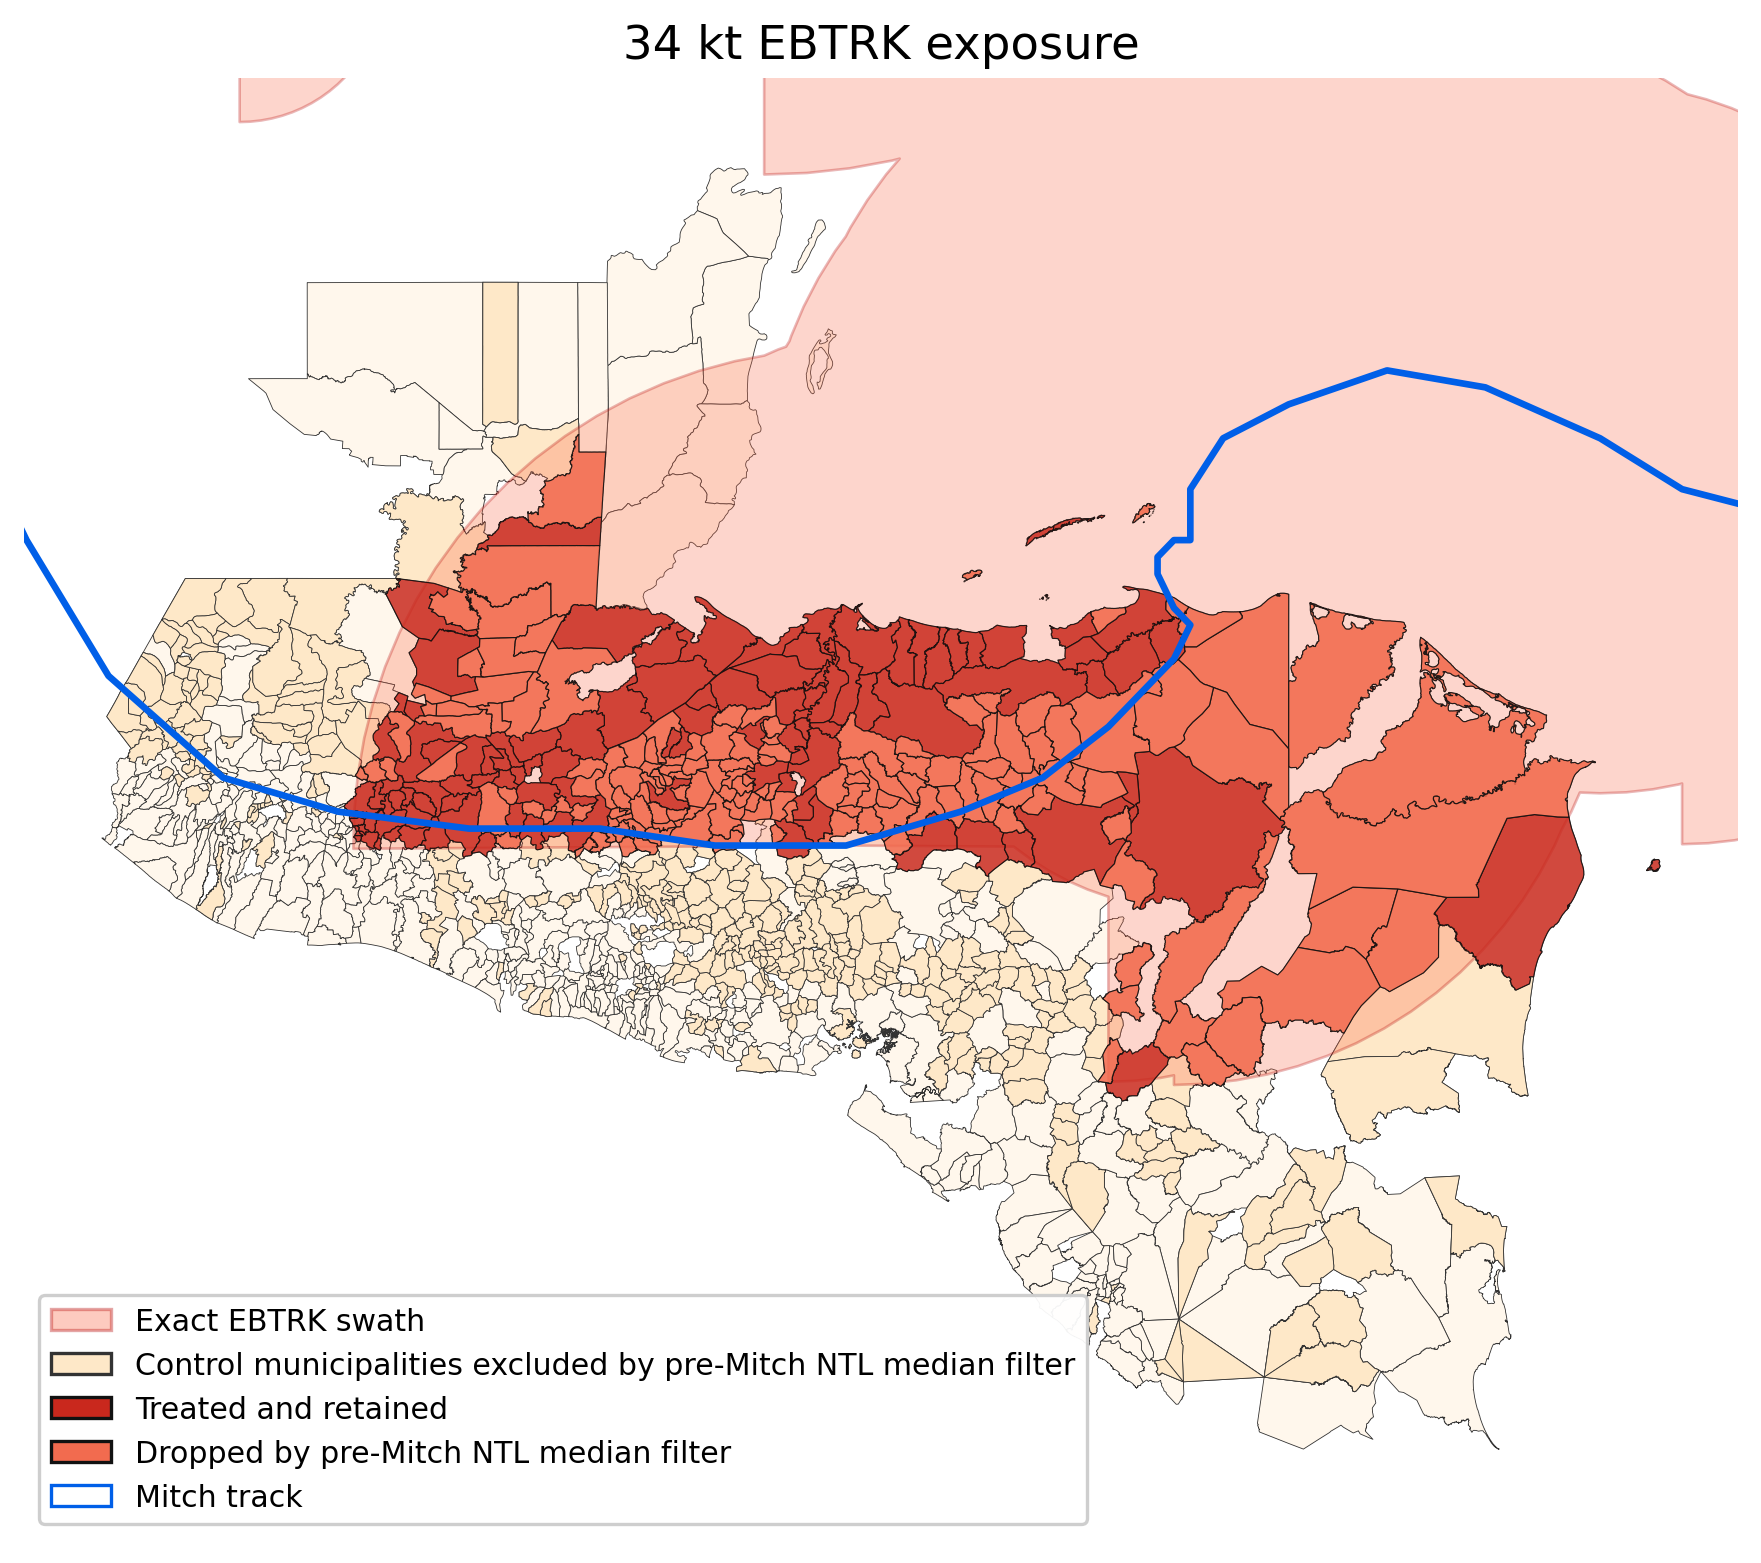
\includegraphics[height=0.34\textheight,keepaspectratio]{Paper_Figures/data/exposure_maps/map_34kt.png}

\vspace{0.3em}
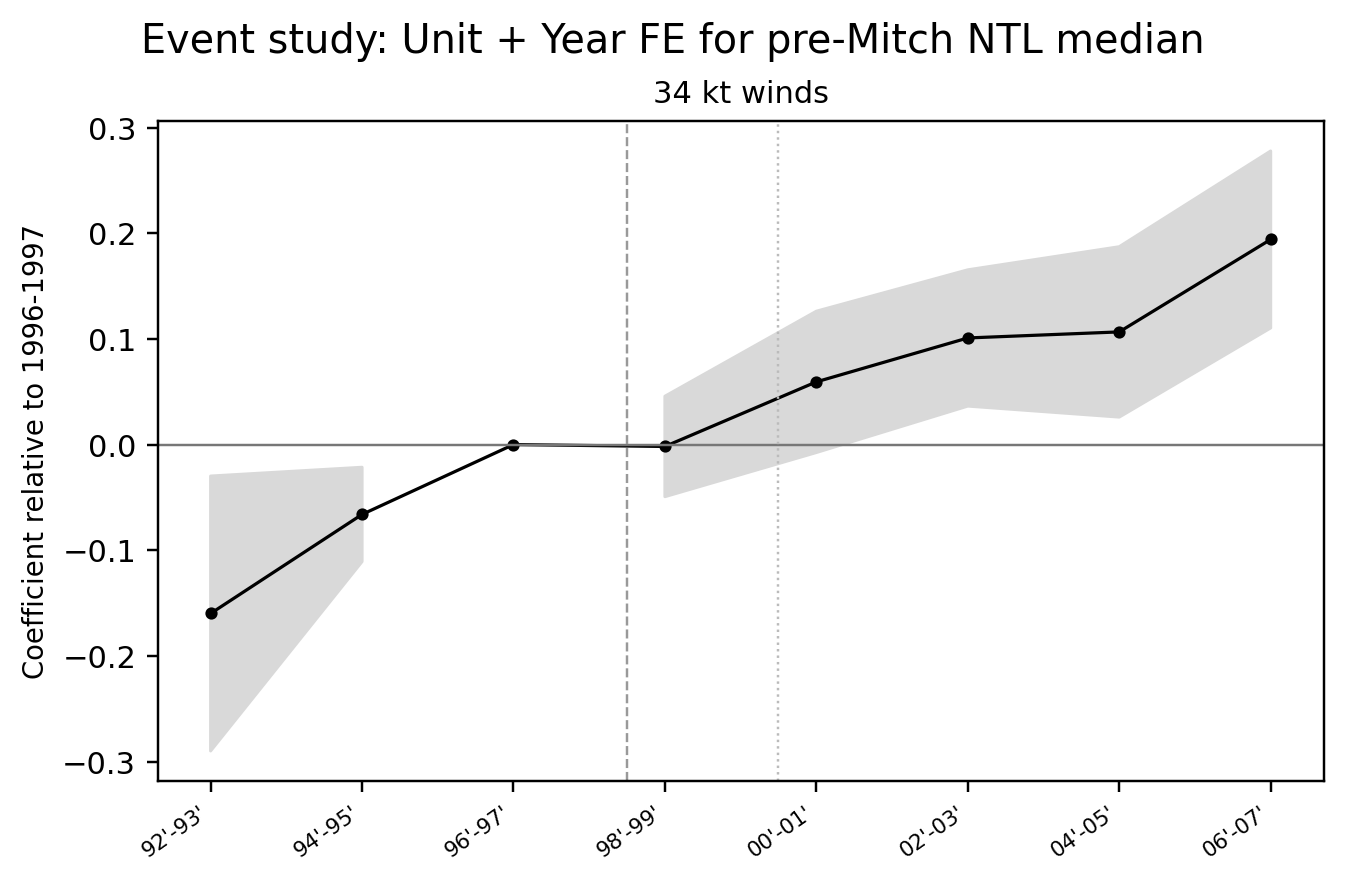
\includegraphics[height=0.34\textheight,keepaspectratio]{Paper_Figures/main_results/figures/event_study/year_fe_ntl_filter/fig_34kt.png}
\widefigurenotes{The top panel maps 34-knot EBTRK exposure. \textbf{The bottom panel reports the Unit + Year FE event-study coefficients for the pre-Mitch median luminosity sample; the omitted period is 1996--1997.} This appendix figure is included as a broad-exposure robustness display.}
\end{figure}

\section{Annual Event-Study Specifications}
\begin{figure}[p]
\centering
\caption{\label{fig:appendix-annual-event-study}Annual event-study coefficients for the main treatment definitions}
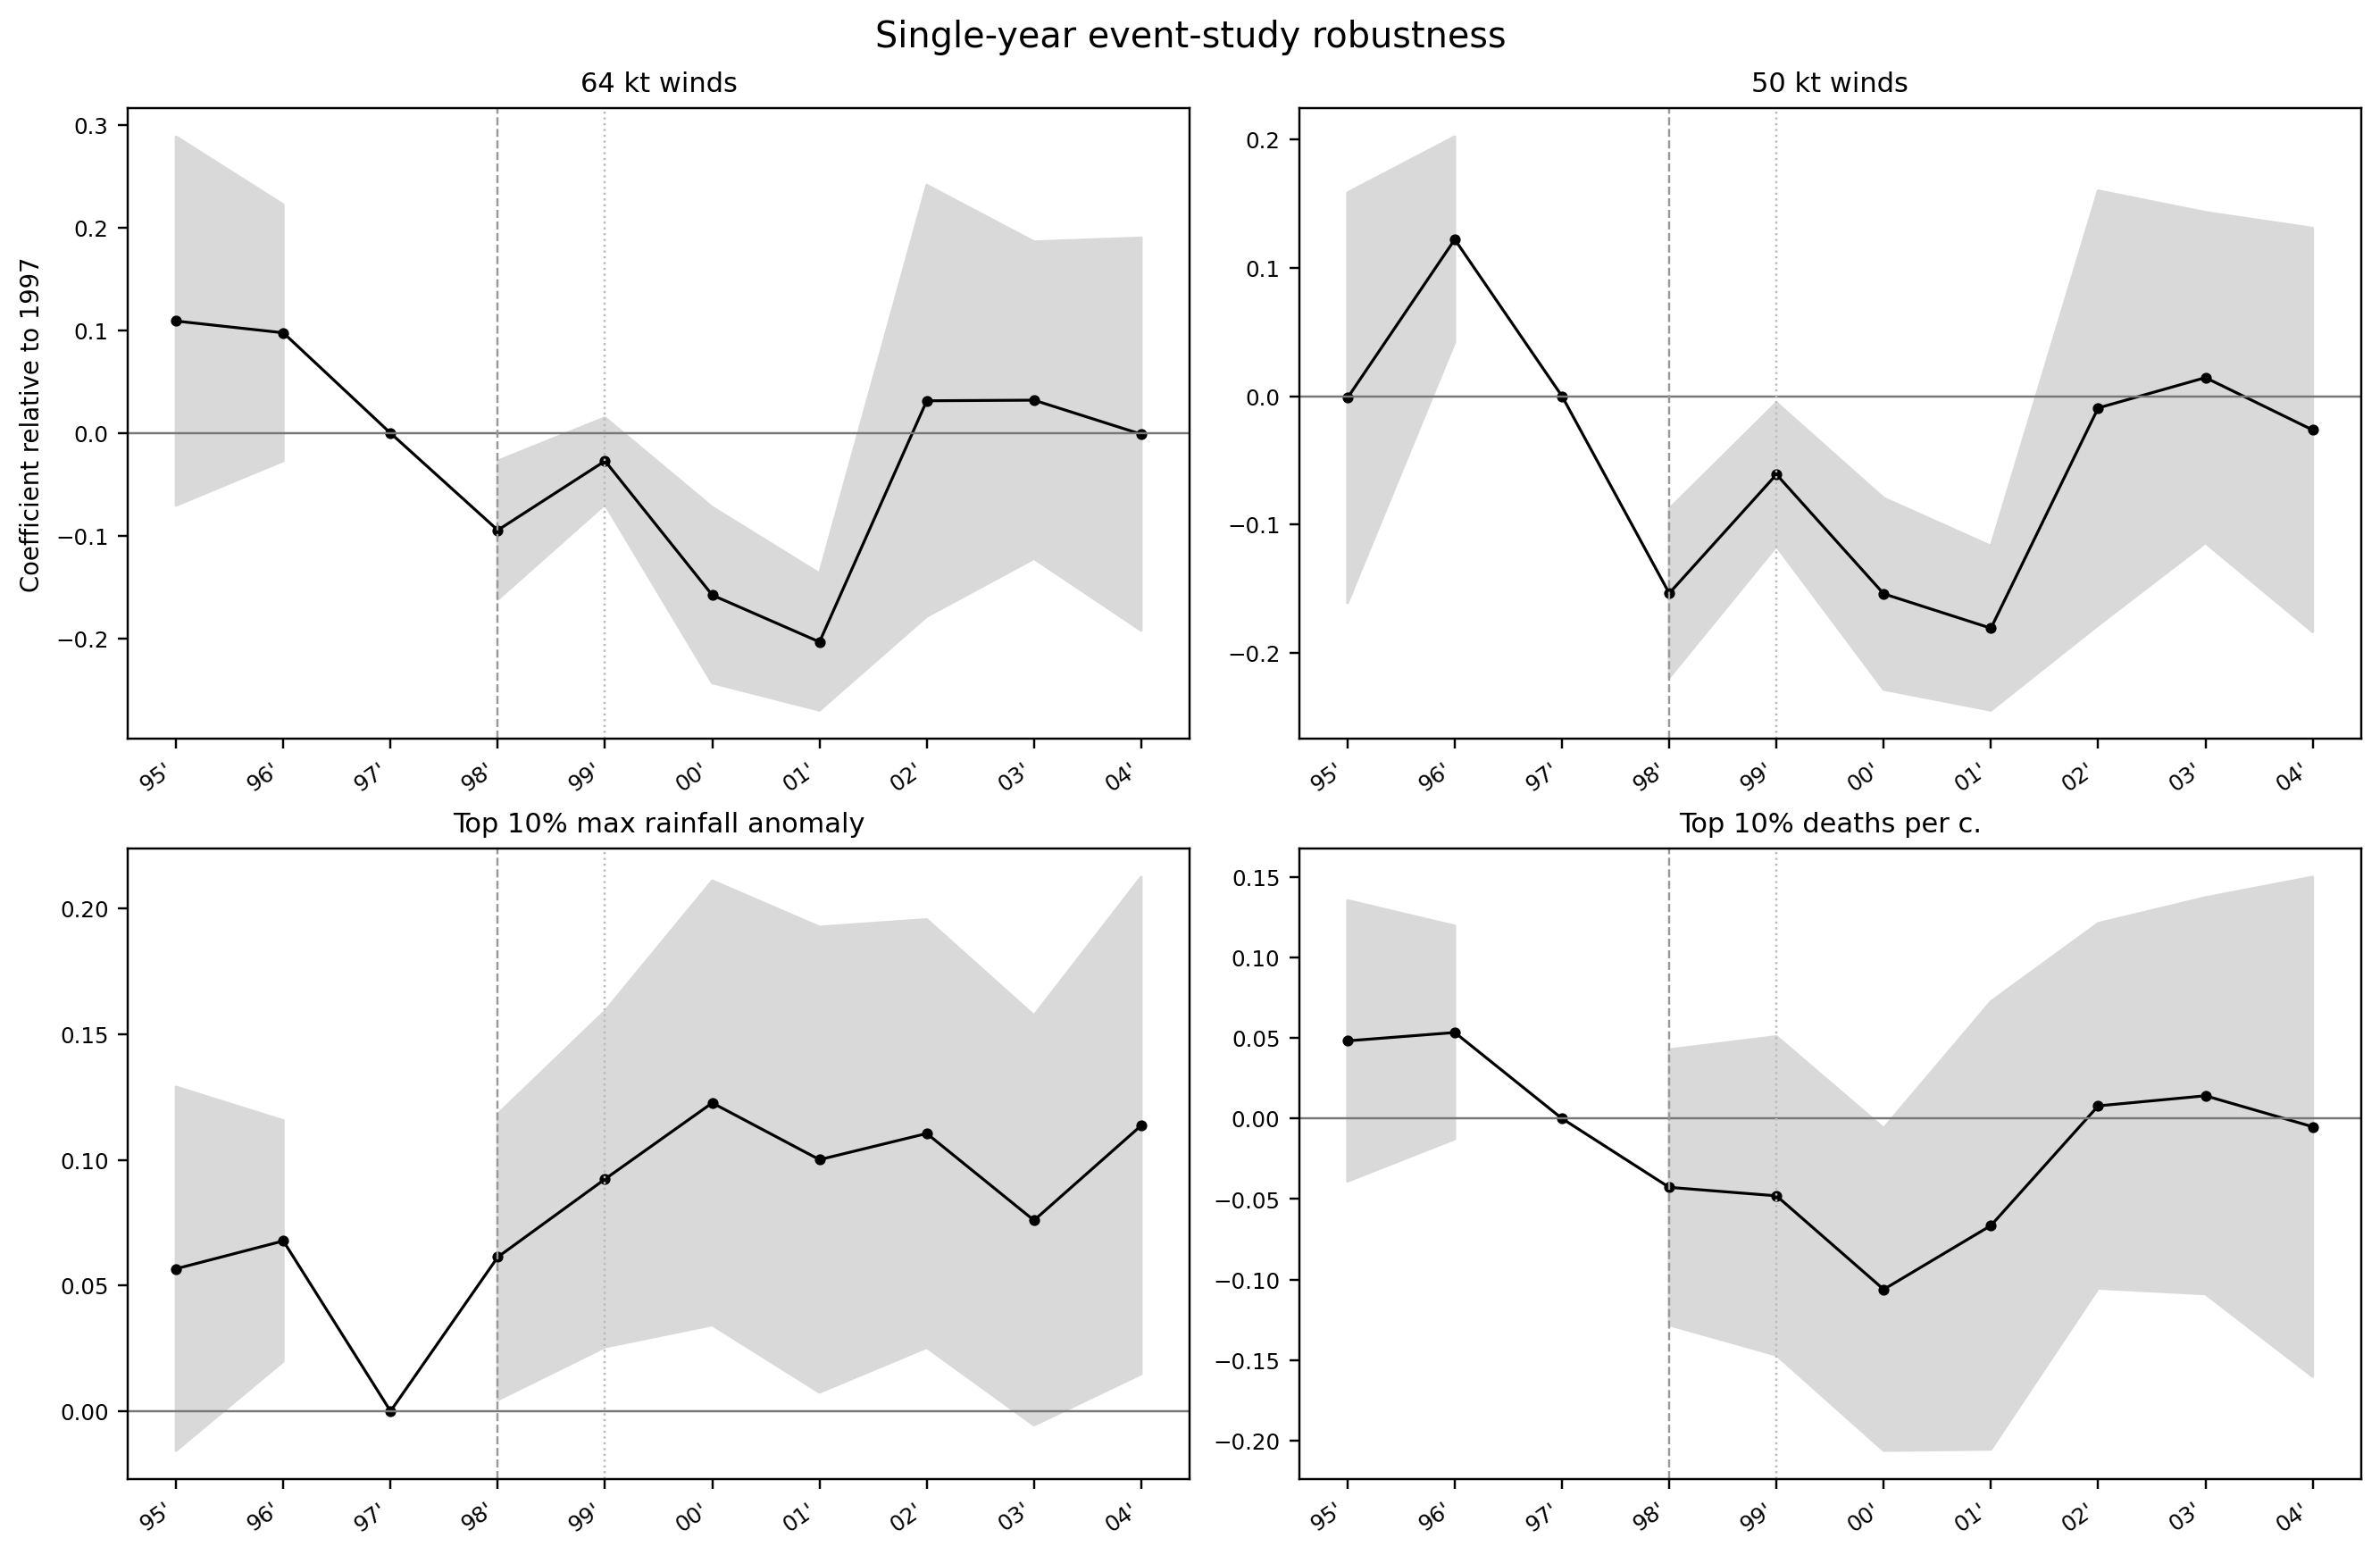
\includegraphics[width=0.96\linewidth]{Paper_Figures/single_years/eventstudy_annual_four_treatments_no34.png}
\widefigurenotes{The figure reports annual Unit + Year FE event-study coefficients for the 64-knot, 50-knot, top-decile rainfall, and top-decile deaths-per-capita treatments. The omitted year is 1997. The annual estimates preserve the delayed 2000 relative loss visible in the two-year specifications.}
\end{figure}

\begin{table}[p]
\centering
\caption{\label{tab:appendix-annual-reg}Annual coefficients for the main treatment definitions}
\begingroup
\scriptsize
\setlength{\tabcolsep}{2pt}
\resizebox{\linewidth}{!}{%
\begin{tabular}{llrrrrrrrrrr}
\toprule
Treatment & Specification & 95' & 96' & 97' & 98' & 99' & 00' & 01' & 02' & 03' & 04' \\
\midrule
64 kt & Unit + Year FE & \begin{tabular}{@{}c@{}}0.260***\\{\scriptsize (0.076)}\end{tabular} & \begin{tabular}{@{}c@{}}0.578*\\{\scriptsize (0.347)}\end{tabular} & ref. & \cellcolor{gray!11}\begin{tabular}{@{}c@{}}-0.105\\{\scriptsize (0.322)}\end{tabular} & \cellcolor{gray!11}\begin{tabular}{@{}c@{}}-0.483\\{\scriptsize (0.725)}\end{tabular} & \cellcolor{gray!11}\begin{tabular}{@{}c@{}}-0.200\\{\scriptsize (0.479)}\end{tabular} & \cellcolor{gray!11}\begin{tabular}{@{}c@{}}-0.274\\{\scriptsize (0.480)}\end{tabular} & \cellcolor{gray!11}\begin{tabular}{@{}c@{}}-0.059\\{\scriptsize (0.504)}\end{tabular} & \cellcolor{gray!11}\begin{tabular}{@{}c@{}}-0.025\\{\scriptsize (0.491)}\end{tabular} & \cellcolor{gray!11}\begin{tabular}{@{}c@{}}-0.217\\{\scriptsize (0.478)}\end{tabular} \\
 & \begin{tabular}{@{}l@{}}Unit + Year FE\\for pre-Mitch NTL median\end{tabular} & \begin{tabular}{@{}c@{}}0.109\\{\scriptsize (0.092)}\end{tabular} & \begin{tabular}{@{}c@{}}0.098\\{\scriptsize (0.064)}\end{tabular} & ref. & \cellcolor{gray!39}\begin{tabular}{@{}c@{}}-0.094***\\{\scriptsize (0.034)}\end{tabular} & \cellcolor{gray!11}\begin{tabular}{@{}c@{}}-0.027\\{\scriptsize (0.021)}\end{tabular} & \cellcolor{gray!39}\begin{tabular}{@{}c@{}}-0.158***\\{\scriptsize (0.044)}\end{tabular} & \cellcolor{gray!39}\begin{tabular}{@{}c@{}}-0.203***\\{\scriptsize (0.034)}\end{tabular} & \begin{tabular}{@{}c@{}}0.032\\{\scriptsize (0.107)}\end{tabular} & \begin{tabular}{@{}c@{}}0.032\\{\scriptsize (0.079)}\end{tabular} & \cellcolor{gray!11}\begin{tabular}{@{}c@{}}-0.001\\{\scriptsize (0.097)}\end{tabular} \\
\addlinespace
50 kt & Unit + Year FE & \begin{tabular}{@{}c@{}}0.239***\\{\scriptsize (0.065)}\end{tabular} & \begin{tabular}{@{}c@{}}0.550**\\{\scriptsize (0.241)}\end{tabular} & ref. & \cellcolor{gray!11}\begin{tabular}{@{}c@{}}-0.202\\{\scriptsize (0.197)}\end{tabular} & \cellcolor{gray!11}\begin{tabular}{@{}c@{}}-0.469\\{\scriptsize (0.411)}\end{tabular} & \cellcolor{gray!11}\begin{tabular}{@{}c@{}}-0.356\\{\scriptsize (0.276)}\end{tabular} & \cellcolor{gray!21}\begin{tabular}{@{}c@{}}-0.466*\\{\scriptsize (0.279)}\end{tabular} & \begin{tabular}{@{}c@{}}0.061\\{\scriptsize (0.353)}\end{tabular} & \begin{tabular}{@{}c@{}}0.084\\{\scriptsize (0.353)}\end{tabular} & \cellcolor{gray!11}\begin{tabular}{@{}c@{}}-0.209\\{\scriptsize (0.333)}\end{tabular} \\
 & \begin{tabular}{@{}l@{}}Unit + Year FE\\for pre-Mitch NTL median\end{tabular} & \begin{tabular}{@{}c@{}}-0.001\\{\scriptsize (0.081)}\end{tabular} & \begin{tabular}{@{}c@{}}0.122***\\{\scriptsize (0.041)}\end{tabular} & ref. & \cellcolor{gray!39}\begin{tabular}{@{}c@{}}-0.153***\\{\scriptsize (0.033)}\end{tabular} & \cellcolor{gray!30}\begin{tabular}{@{}c@{}}-0.061**\\{\scriptsize (0.028)}\end{tabular} & \cellcolor{gray!39}\begin{tabular}{@{}c@{}}-0.154***\\{\scriptsize (0.038)}\end{tabular} & \cellcolor{gray!39}\begin{tabular}{@{}c@{}}-0.181***\\{\scriptsize (0.033)}\end{tabular} & \cellcolor{gray!11}\begin{tabular}{@{}c@{}}-0.009\\{\scriptsize (0.086)}\end{tabular} & \begin{tabular}{@{}c@{}}0.014\\{\scriptsize (0.066)}\end{tabular} & \cellcolor{gray!11}\begin{tabular}{@{}c@{}}-0.026\\{\scriptsize (0.080)}\end{tabular} \\
\addlinespace
Top 10\% rain & Unit + Year FE & \begin{tabular}{@{}c@{}}0.122\\{\scriptsize (0.101)}\end{tabular} & \begin{tabular}{@{}c@{}}0.165**\\{\scriptsize (0.075)}\end{tabular} & ref. & \cellcolor{gray!39}\begin{tabular}{@{}c@{}}-0.206***\\{\scriptsize (0.054)}\end{tabular} & \cellcolor{gray!11}\begin{tabular}{@{}c@{}}-0.049\\{\scriptsize (0.087)}\end{tabular} & \cellcolor{gray!11}\begin{tabular}{@{}c@{}}-0.018\\{\scriptsize (0.099)}\end{tabular} & \cellcolor{gray!11}\begin{tabular}{@{}c@{}}-0.074\\{\scriptsize (0.116)}\end{tabular} & \cellcolor{gray!11}\begin{tabular}{@{}c@{}}-0.059\\{\scriptsize (0.108)}\end{tabular} & \cellcolor{gray!11}\begin{tabular}{@{}c@{}}-0.115\\{\scriptsize (0.094)}\end{tabular} & \cellcolor{gray!11}\begin{tabular}{@{}c@{}}-0.123\\{\scriptsize (0.126)}\end{tabular} \\
 & \begin{tabular}{@{}l@{}}Unit + Year FE\\for pre-Mitch NTL median\end{tabular} & \begin{tabular}{@{}c@{}}0.057\\{\scriptsize (0.037)}\end{tabular} & \begin{tabular}{@{}c@{}}0.068***\\{\scriptsize (0.024)}\end{tabular} & ref. & \begin{tabular}{@{}c@{}}0.061**\\{\scriptsize (0.029)}\end{tabular} & \begin{tabular}{@{}c@{}}0.092***\\{\scriptsize (0.034)}\end{tabular} & \begin{tabular}{@{}c@{}}0.123***\\{\scriptsize (0.045)}\end{tabular} & \begin{tabular}{@{}c@{}}0.100**\\{\scriptsize (0.047)}\end{tabular} & \begin{tabular}{@{}c@{}}0.110**\\{\scriptsize (0.043)}\end{tabular} & \begin{tabular}{@{}c@{}}0.076*\\{\scriptsize (0.042)}\end{tabular} & \begin{tabular}{@{}c@{}}0.114**\\{\scriptsize (0.050)}\end{tabular} \\
\addlinespace
Top 10\% deaths per c. & Unit + Year FE & \begin{tabular}{@{}c@{}}0.031\\{\scriptsize (0.048)}\end{tabular} & \begin{tabular}{@{}c@{}}0.043\\{\scriptsize (0.035)}\end{tabular} & ref. & \cellcolor{gray!11}\begin{tabular}{@{}c@{}}-0.049\\{\scriptsize (0.044)}\end{tabular} & \cellcolor{gray!11}\begin{tabular}{@{}c@{}}-0.057\\{\scriptsize (0.051)}\end{tabular} & \cellcolor{gray!30}\begin{tabular}{@{}c@{}}-0.123**\\{\scriptsize (0.053)}\end{tabular} & \cellcolor{gray!11}\begin{tabular}{@{}c@{}}-0.088\\{\scriptsize (0.074)}\end{tabular} & \cellcolor{gray!11}\begin{tabular}{@{}c@{}}-0.005\\{\scriptsize (0.059)}\end{tabular} & \cellcolor{gray!11}\begin{tabular}{@{}c@{}}-0.003\\{\scriptsize (0.065)}\end{tabular} & \cellcolor{gray!11}\begin{tabular}{@{}c@{}}-0.027\\{\scriptsize (0.082)}\end{tabular} \\
 & \begin{tabular}{@{}l@{}}Unit + Year FE\\for pre-Mitch NTL median\end{tabular} & \begin{tabular}{@{}c@{}}0.048\\{\scriptsize (0.044)}\end{tabular} & \begin{tabular}{@{}c@{}}0.053\\{\scriptsize (0.034)}\end{tabular} & ref. & \cellcolor{gray!11}\begin{tabular}{@{}c@{}}-0.043\\{\scriptsize (0.044)}\end{tabular} & \cellcolor{gray!11}\begin{tabular}{@{}c@{}}-0.048\\{\scriptsize (0.050)}\end{tabular} & \cellcolor{gray!30}\begin{tabular}{@{}c@{}}-0.106**\\{\scriptsize (0.051)}\end{tabular} & \cellcolor{gray!11}\begin{tabular}{@{}c@{}}-0.066\\{\scriptsize (0.071)}\end{tabular} & \begin{tabular}{@{}c@{}}0.008\\{\scriptsize (0.058)}\end{tabular} & \begin{tabular}{@{}c@{}}0.014\\{\scriptsize (0.063)}\end{tabular} & \cellcolor{gray!11}\begin{tabular}{@{}c@{}}-0.005\\{\scriptsize (0.079)}\end{tabular} \\
\bottomrule
\end{tabular}

}
\endgroup
\tablenotes{The outcome is log(1 + DMSP-OLS stable lights). Rows report Unit + Year FE specifications with and without the pre-Mitch median luminosity filter. The omitted year is 1997, and standard errors are clustered by the estimation unit.}
\end{table}

\section{Unit-Fixed-Effects Regression Table}
Table \ref{tab:appendix-unit-fe-reg} reports the Unit-FE coefficients underlying Figure \ref{fig:unit-fe-dynamic}.

\begin{table}[p]
\centering
\caption{\label{tab:appendix-unit-fe-reg}Two-year coefficients with unit fixed effects}
\begingroup
\scriptsize
\setlength{\tabcolsep}{3pt}
\resizebox{\linewidth}{!}{%
\begin{tabular}{llrrrrrrrrr}
\toprule
Treatment & Specification & 92'-93' & 94'-95' & 96'-97' & 98'-99' & 00'-01' & 02'-03' & 04'-05' & 06'-07' & 08'-09'$\ldots$ \\
\midrule
64 kt & Unit FE & \begin{tabular}{@{}c@{}}-1.172***\\{\scriptsize (0.312)}\end{tabular} & \begin{tabular}{@{}c@{}}-0.597***\\{\scriptsize (0.178)}\end{tabular} & ref. & \begin{tabular}{@{}c@{}}0.005\\{\scriptsize (0.559)}\end{tabular} & \begin{tabular}{@{}c@{}}0.397\\{\scriptsize (0.549)}\end{tabular} & \begin{tabular}{@{}c@{}}0.502\\{\scriptsize (0.571)}\end{tabular} & \begin{tabular}{@{}c@{}}0.482\\{\scriptsize (0.528)}\end{tabular} & \begin{tabular}{@{}c@{}}0.613\\{\scriptsize (0.545)}\end{tabular} & \begin{tabular}{@{}c@{}}0.548\\{\scriptsize (0.568)}\end{tabular} \\
\addlinespace
50 kt & Unit FE & \begin{tabular}{@{}c@{}}-1.436***\\{\scriptsize (0.302)}\end{tabular} & \begin{tabular}{@{}c@{}}-0.722***\\{\scriptsize (0.164)}\end{tabular} & ref. & \cellcolor{gray!11}\begin{tabular}{@{}c@{}}-0.017\\{\scriptsize (0.331)}\end{tabular} & \begin{tabular}{@{}c@{}}0.243\\{\scriptsize (0.326)}\end{tabular} & \begin{tabular}{@{}c@{}}0.630*\\{\scriptsize (0.354)}\end{tabular} & \begin{tabular}{@{}c@{}}0.531*\\{\scriptsize (0.318)}\end{tabular} & \begin{tabular}{@{}c@{}}0.466\\{\scriptsize (0.329)}\end{tabular} & \begin{tabular}{@{}c@{}}0.496\\{\scriptsize (0.321)}\end{tabular} \\
\addlinespace
Top 10\% rain & Unit FE & \begin{tabular}{@{}c@{}}-0.934***\\{\scriptsize (0.108)}\end{tabular} & \begin{tabular}{@{}c@{}}-0.366***\\{\scriptsize (0.074)}\end{tabular} & ref. & \begin{tabular}{@{}c@{}}0.393***\\{\scriptsize (0.048)}\end{tabular} & \begin{tabular}{@{}c@{}}0.801***\\{\scriptsize (0.089)}\end{tabular} & \begin{tabular}{@{}c@{}}0.676***\\{\scriptsize (0.084)}\end{tabular} & \begin{tabular}{@{}c@{}}0.872***\\{\scriptsize (0.107)}\end{tabular} & \begin{tabular}{@{}c@{}}0.861***\\{\scriptsize (0.107)}\end{tabular} & \begin{tabular}{@{}c@{}}0.955***\\{\scriptsize (0.121)}\end{tabular} \\
\addlinespace
Top 10\% deaths per c. & Unit FE & \begin{tabular}{@{}c@{}}-0.571***\\{\scriptsize (0.068)}\end{tabular} & \begin{tabular}{@{}c@{}}-0.205***\\{\scriptsize (0.031)}\end{tabular} & ref. & \begin{tabular}{@{}c@{}}0.213***\\{\scriptsize (0.041)}\end{tabular} & \begin{tabular}{@{}c@{}}0.413***\\{\scriptsize (0.054)}\end{tabular} & \begin{tabular}{@{}c@{}}0.411***\\{\scriptsize (0.052)}\end{tabular} & \begin{tabular}{@{}c@{}}0.499***\\{\scriptsize (0.074)}\end{tabular} & \begin{tabular}{@{}c@{}}0.633***\\{\scriptsize (0.102)}\end{tabular} & \begin{tabular}{@{}c@{}}0.659***\\{\scriptsize (0.086)}\end{tabular} \\
\bottomrule
\end{tabular}

}
\endgroup
\tablenotes{The outcome is log(1 + DMSP-OLS stable lights). \textbf{All rows include unit fixed effects but not calendar-year fixed effects or the pre-Mitch median luminosity filter.} The 1996--1997 treatment interaction is omitted, and standard errors are clustered by the estimation unit.}
\end{table}

\section{Honduran Census Robustness}
\begin{table}[p]
\centering
\caption{\label{tab:appendix-ipums-expanded}Expanded population, education, worker type, and dwelling conditions in Honduran 50-knot census groups}
\begingroup
\scriptsize
\setlength{\tabcolsep}{3pt}
\textbf{Panel A. Population, adult education, and class of worker in census years}
\par\smallskip
\resizebox{\linewidth}{!}{%
\begin{tabular}{lcrrrrrrrrrr}
\toprule
 & & \multicolumn{3}{c}{Population (thousands)} & \multicolumn{3}{c}{Mean school years, age 25+} & \multicolumn{3}{c}{CLASSWK: self-employed / wage-salary (\%), age 15+} \\
\cmidrule(lr){3-5}\cmidrule(lr){6-8}\cmidrule(lr){9-11}
IPUMS geography & 50-kt coverage & 1988 & 2001 & 2013 & 1988 & 2001 & 2013 & 1988 & 2001 & 2013 \\
\midrule
Colon group: Balfate--Iriona & 7/7 & 66.5 & 112.2 & 148.9 & 2.5 & 3.5 & 4.7 & 60.9 / 36.2 & 44.8 / 42.7 & 27.6 / 48.2 \\
Colon group: Saba--Tocoa & 3/3 & 78.0 & 107.3 & 163.8 & 2.7 & 4.1 & 5.3 & 50.3 / 46.7 & 39.0 / 49.6 & 29.9 / 52.8 \\
Gracias a Dios group & 1/6 & 33.2 & 57.5 & 89.5 & 2.7 & 3.9 & 5.0 & 50.4 / 40.4 & 52.7 / 21.9 & 43.7 / 21.8 \\
Bay Islands group & 3/4 & 21.5 & 31.2 & 63.7 & 4.6 & 6.2 & 7.0 & 24.9 / 74.5 & 22.4 / 72.4 & 19.1 / 68.8 \\
Olancho group: Gualaco--San Esteban & 2/2 & 24.6 & 37.7 & 47.2 & 1.7 & 3.0 & 4.2 & 76.5 / 19.0 & 53.8 / 28.6 & 34.1 / 37.6 \\
Honduras &  & 4,239.7 & 6,086.2 & 8,303.1 & 3.4 & 4.8 & 5.7 & 42.6 / 53.3 & 38.2 / 50.5 & 34.4 / 52.6 \\
\bottomrule
\end{tabular}%
}
\par\medskip
\textbf{Panel B. Household-weighted dwelling characteristics}
\par\smallskip
\resizebox{\linewidth}{!}{%
\begin{tabular}{lrrrrrr}
\toprule
 & \multicolumn{2}{c}{1988} & \multicolumn{2}{c}{2001} & \multicolumn{2}{c}{2013} \\
\cmidrule(lr){2-3}\cmidrule(lr){4-5}\cmidrule(lr){6-7}
Characteristic (\% of households) & Treated & Honduras & Treated & Honduras & Treated & Honduras \\
\midrule
Electricity & 23.2 & 39.6 & 48.6 & 60.2 & 78.2 & 80.8 \\
Piped water & 54.5 & 66.1 & 77.6 & 80.4 & 87.4 & 86.1 \\
Sewer or septic & 11.2 & 26.7 & 41.9 & 50.8 & 74.8 & 68.7 \\
Wood or other solid cooking fuel & 90.2 & 74.3 & 71.6 & 59.1 & 60.1 & 54.5 \\
Earth floor & 62.9 & 51.1 & 35.5 & 33.5 & 19.1 & 22.9 \\
Masonry wall & 18.2 & 24.6 & 55.4 & 46.6 & 68.9 & 53.8 \\
Sheet-metal roof & 41.6 & 38.4 & 61.1 & 47.9 & 83.3 & 63.7 \\
Refrigerator & 12.2 & 19.3 & 28.2 & 34.5 & 57.5 & 59.4 \\
Television & 5.5 & 29.3 & 30.3 & 47.9 & 61.4 & 67.1 \\
More than three persons per room & 37.7 & 30.6 & 21.3 & 17.0 & 10.9 & 9.2 \\
\bottomrule
\end{tabular}%
}

\endgroup
\tablenotes{This is the expanded version of Table \ref{tab:ipums-resilience}. Panel A retains CLASSWK self-employed and wage-salary shares, and Panel B reports the wider set of household and dwelling characteristics available in 1988, 2001, and 2013. Mixed harmonized groups are descriptive only; the preferred DiDs use the three clean groups containing 12 treated municipalities and no untreated municipalities. Source: IPUMS International and author's calculations \parencite{ipumsinternational2025}.}
\end{table}

\begin{figure}[p]
\centering
\caption{\label{fig:appendix-normal-goods}Census normal-goods event study}
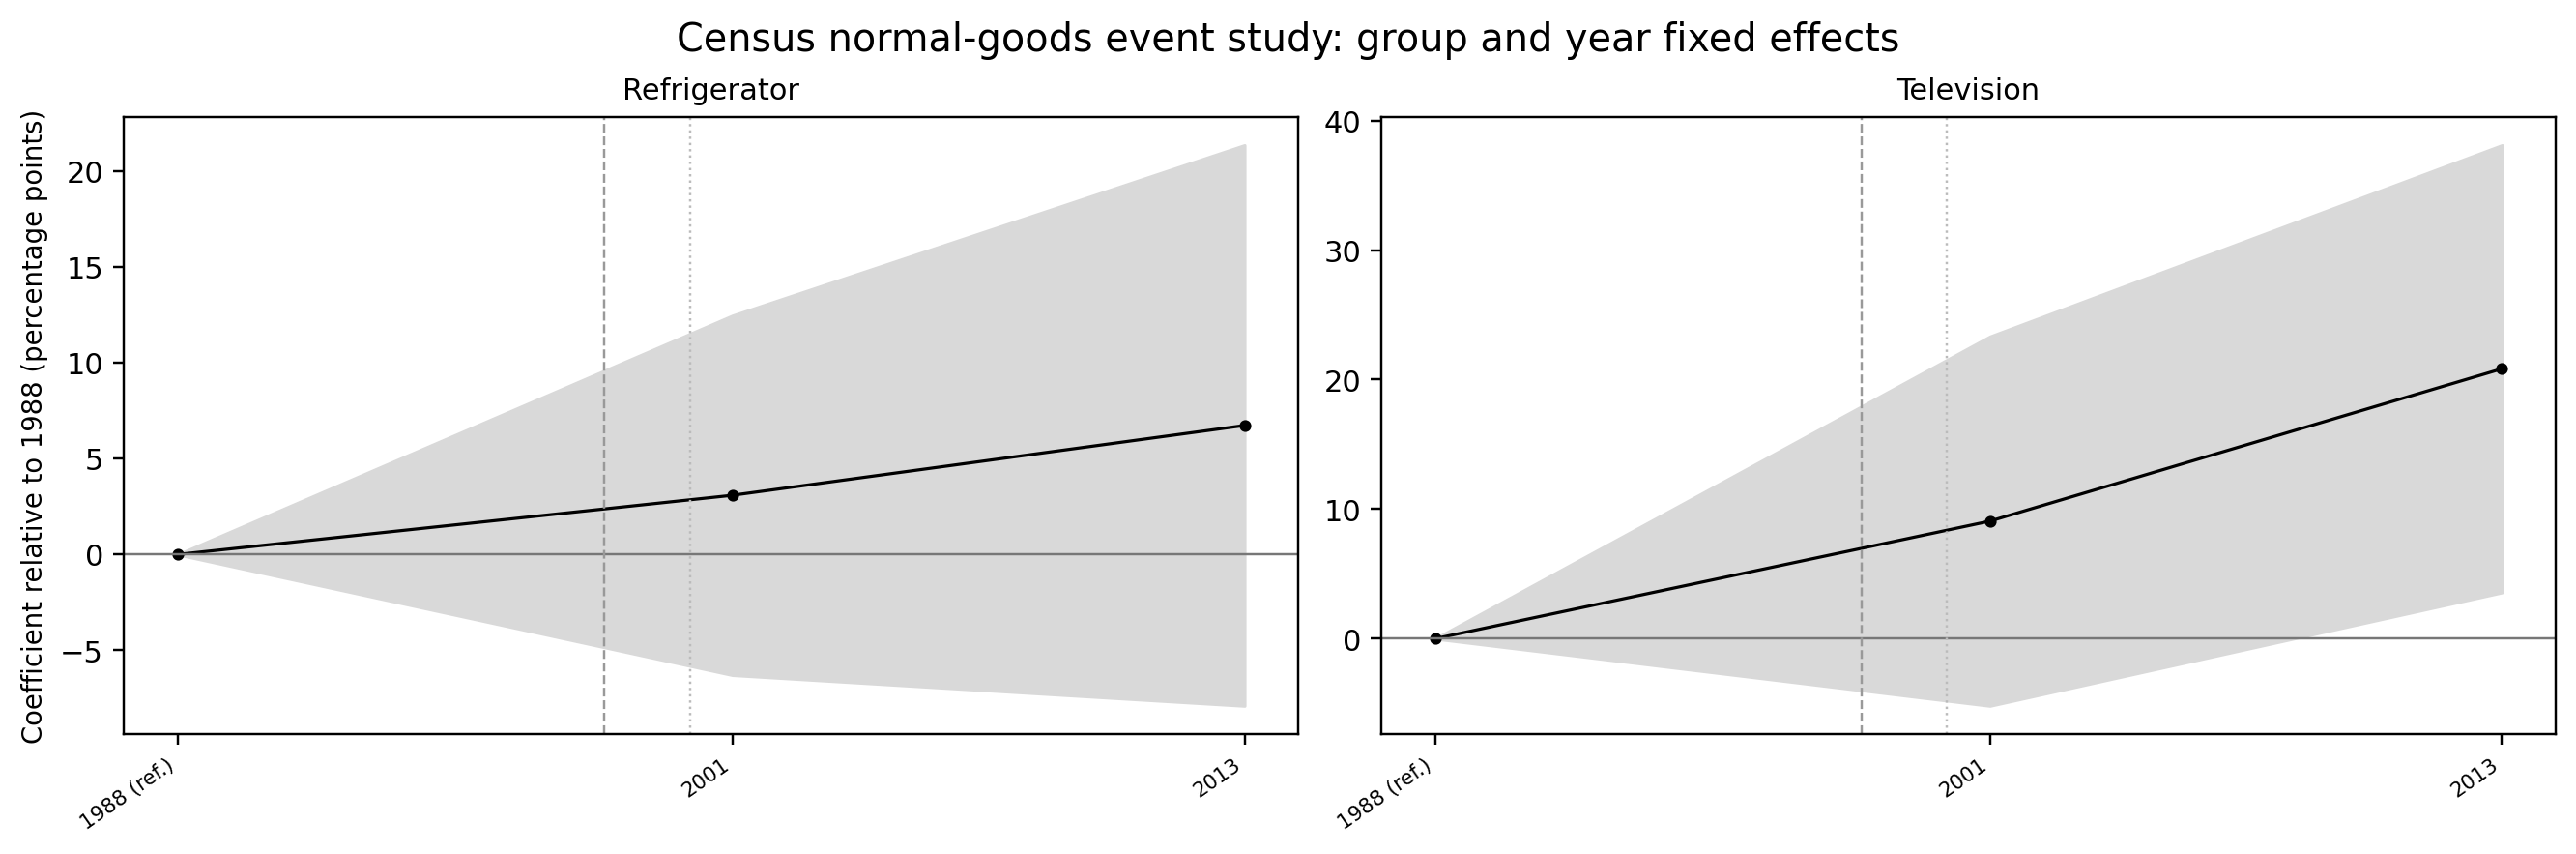
\includegraphics[width=0.96\linewidth]{Paper_Figures/appendix/census/normal_goods_did_event_studies.png}
\widefigurenotes{The panels follow the visual logic of the main event-study figure and report coefficients relative to the omitted 1988 census for refrigerator and television ownership. Models include harmonized-group and census-year fixed effects, use household weights, and cluster standard errors by harmonized group. Gracias a Dios and the mixed Bay Islands group are excluded. The 1974 census is not plotted because these household assets are not reported in that sample.}
\end{figure}

\begin{table}[htbp]
\centering
\caption{Normal-goods census DiD estimates (percentage points)}
\label{tab:normal-goods}
\resizebox{\linewidth}{!}{%
\begin{tabular}{lrrrrrr}
\toprule
Specification & Outcome & Term & Estimate & SE & Cells & Clusters \\
\midrule
clean & refrigerator & treated\_x\_2001 & 3.088 & 4.785 & 297 & 99 \\
clean & refrigerator & treated\_x\_2013 & 6.731 & 7.462 & 297 & 99 \\
clean & television & treated\_x\_2001 & 9.074 & 7.273 & 297 & 99 \\
clean & television & treated\_x\_2013 & 20.837 & 8.809 & 297 & 99 \\
\bottomrule
\end{tabular}%
}
\end{table}


\clearpage
\printbibliography

\end{document}
